% !TEX root = ../main.tex

\section{Combinatorial semantics}


\update{Below I will assume that we work with a simple PROP (not coloured)}

Before we begin we first fix some notation.
When $V$ is a set, we denote with $V^{*}$ a set of all finite sequences of the elements of $V$, i.e. $^*$ is a free monoid.
When $\phi : V \to V'$ is a function, we denote with $\phi^{*}$ an extension of $\phi$ to sequences, i.e. $\phi^{*} : V^* \to V'^{*}$ and it applies $\phi$ element-wise.
Similarly, in the case when $\psi \subset V \times V$ is a relation: we denote with $\psi^{*}: \subset V^* \times V^*$ the element-wise relation on ordered sequences.
We will denote with $A +_{f,g} B$ the pushout of $A \xleftarrow{f} C \xrightarrow{g} B$.

There was a correspondence between hypergraphs and terms in $\textsf{PROP}(\Sigma)$ developed in~\cite{Frobenius, Frobenius2} which we will refer to throughout this section. We first recall the notion of a hypergraph from there.

\Aleksei{Actually, in~\cite{Frobenius} a hypergraph is defined as an object of the corresponding category and labelled hypergraphs are defined as a slice category. This is needed to show adhesiveness. As our category is not adhesive, I think we can follow a more straightforward definition of a tuple.}

\begin{definition}[Category $\catname{Hyp_{\Sigma}}$]


A hypergraph $\mathcal{G}_{\Sigma}$ over a monoidal signature $\Sigma$ is a tuple 
\[
(V_{\mathcal{G}},E_{\mathcal{G}},s,t,l)
\]
\label{def:hypergraph}

where $V_{\mathcal{G}}$ is the set of nodes, $E_{\mathcal{G}}$ is a set of edges, $s : E_{\mathcal{G}} \to V_{\mathcal{G}}^{*}$ is a source function that for each edge returns the ordered list of the edge's source nodes, $t : E_{\mathcal{G}} \to V_{\mathcal{G}}^{*}$ is a target function that for each edge returns the ordered list of the edge's target nodes, $l : E_{\mathcal{G}} \to \Sigma$ is a label function that labels each edge with a generator from monoidal signature $\Sigma$. The label function should satisfy the following conditions: $\forall e,\; \text{s.t.}\; l(e) : m \to n\;. \;|s(e)| = m$ and $\forall e,\; \text{s.t.}\; l(e) : m \to n \;. \;|t(e)| = n$

We will omit the subscripts when they are clear from the context.

A homomorphism $\phi: \mathcal{F} \to \mathcal{G}$ of hypergraphs $\mathcal{F},\mathcal{G}$ is a pair of functions $\phi_V : V_{\mathcal{F}} \to V_{\mathcal{G}}, \phi_E : E_{\mathcal{F}} \to E_{\mathcal{G}}$ such that

\begin{enumerate}
        \item $(s_{\mathcal{F}};\phi_V^*)(e) = (\phi_E;s_{\mathcal{G}})(e)$
    \item $(t_{\mathcal{F}};\phi_V^*)(e) = (\phi_E;t_{\mathcal{G}})(e)$
    \item $l_{\mathcal{F}}(e) = \phi_E;l_{\mathcal{G}}(e)$
\end{enumerate}


Hypergraphs over a monoidal signature $\Sigma$ together with hypergraph homomorphisms form a category $\catname{Hyp_{\Sigma}}$. 
\end{definition}

\begin{definition}[Definition 2.10~\cite{Frobenius}]
Let $\mathbb{C}$ be a category with all finite colimits. A cospan from $X$ to $Y$ is a pair of arrows $X \xrightarrow{} A \xleftarrow{} Y$  in $\mathbb{C}$.

Two cospans $X \xrightarrow{} A \xleftarrow{} Y$ and $X \xrightarrow{} B \xleftarrow{} Y$ are isomorphic if the following diagram commutes and $\alpha$ is iso.

\[
\begin{tikzcd}
                                               & A \arrow[dd, "\alpha"] &                                                \\
X \arrow[ru, bend left] \arrow[rd, bend right] &                        & Y \arrow[ld, bend left] \arrow[lu, bend right] \\
                                               & B                      &                                               
\end{tikzcd}
\]


For $X \in \mathbb{C}$ an $id$-cospan is $X \xrightarrow{id_X} X \xleftarrow{id_X} X$.
The composition of cospans $X \xrightarrow{} A \xleftarrow{f} Y$ and $Y \xrightarrow{g} B \xleftarrow{} Z$ is $X \xrightarrow{} A +_{f,g} B \xleftarrow{} Z$, constructed by taking a pushout of $f,g$.
This data is the category $\catname{Csp(\mathbb{C})}$: the objects are those of $\mathbb{C}$ and the arrows are isomorphism classes of cospans.
Finally, $\catname{Csp(\mathbb{C})}$ is a monoidal category: monoidal product is given by a coproduct (denoted with $+$) in $\mathbb{C}$ and the unit is given by the initial object of $\mathcal{C}$ as can be seen below.

% \[
% \adjustbox{scale=0.75,center}{
% https://q.uiver.app/#q=WzAsMTEsWzAsMCwiQSJdLFsxLDAsIlxcbWF0aGNhbHtHfSJdLFsyLDAsIkIiXSxbMywwLCJcXG90aW1lcyJdLFs0LDAsIkEnIl0sWzYsMCwiQiciXSxbNSwwLCJcXG1hdGhjYWx7Ryd9Il0sWzcsMCwiOj0iXSxbOCwwLCJBK0EnIl0sWzEwLDAsIlxcbWF0aGNhbHtHfStcXG1hdGhjYWx7Ryd9Il0sWzEyLDAsIkIrQiciXSxbMCwxLCJmIl0sWzIsMSwiZyIsMl0sWzQsNiwiZiciXSxbNSw2LCJnJyIsMl0sWzgsOSwiZitmJyJdLFsxMCw5LCJnK2cnIiwyXV0=
% \begin{tikzcd}
% 	A & {\mathcal{G}} & B & \otimes & {A'} & {\mathcal{G'}} & {B'} & {:=} & {A+A'} && {\mathcal{G}+\mathcal{G'}} && {B+B'}
% 	\arrow["f", from=1-1, to=1-2]
% 	\arrow["g"', from=1-3, to=1-2]
% 	\arrow["{f'}", from=1-5, to=1-6]
% 	\arrow["{g'}"', from=1-7, to=1-6]
% 	\arrow["{f+f'}", from=1-9, to=1-11]
% 	\arrow["{g+g'}"', from=1-13, to=1-11]
% \end{tikzcd}
\[
    A \xrightarrow{f} \mathcal{G} \xleftarrow{g} B \otimes A' \xrightarrow{f'} \mathcal{G'} \xleftarrow{g'} B' := A + A' \xrightarrow{f'} \mathcal{G} + \mathcal{G'} \xleftarrow{g'} B + B'
\]

Symmetry is inherited from $\mathcal{C}$ as the coproduct is commutative and is given below.

\[
n + m \xrightarrow{\sigma_{n,m}} m + n \xleftarrow{id + id} m + n
\]

Naturality is implied by $+$ being a coproduct~\cite{Frobenius}.

\end{definition}


\begin{remark}
    
Taking isomorphism classes of cospans as morphisms turns $\catname{Csp(\mathbb{C})}$ into a proper category since pushouts are defined up to isomorphism and associative.
\end{remark}

When $\mathbb{C} = \catname{Hyp_{\Sigma}}$ we get a category of cospans of hypergraphs.
$\catname{Hyp_{\Sigma}}$ has all finite colimits and, in particular, coproduct is a disjoint union of two hypergraphs.
An empty hypergraph is the initial object in $Hyp_{\Sigma}$ and coproduct and pushout are defined on the underlying sets of nodes and edges.
Following~\cite{Frobenius2} morphisms in an SMC with a signature $\Sigma$ can be interpreted as particular cospans of hypergraphs. 

\begin{definition}[Category $\;\catname{Csp_{D}(Hyp_{\Sigma})}$]
\label{def:cspd}
Category $\catname{Csp_{D}(Hyp_{\Sigma})}$ is a \textit{full} sub-category of $\catname{Csp(Hyp_{\Sigma})}$ which has discrete hypergraphs as objects.
\end{definition}

In particular, this means that any morphism in $\catname{Csp_{D}(Hyp_{\Sigma})}$ is of the form $n \xrightarrow{} \mathcal{G} \xleftarrow{} m$,
where $n,\;m$ are discrete hypergraphs and $\mathcal{G}$ is an arbitrary hypergraph.
When string diagrams are interpreted as cospans of hypergraphs $n,m$ correspond to input and output interfaces of a string diagram respectively.
A pictorial representation of such a cospan is depicted below in Figure~\ref{fig:hypergraph_and_string_diagram}.
We use node labels to define mappings $n \to \mathcal{F}$ and $m \to \mathcal{F}$.

\begin{figure}
    \centering
    \begin{subfigure}{0.45\linewidth}
    \[
    \scalebox{0.6}{
	\tikzfig{combinatorial_semantics/mda-hypergraph-example}
   }
   \]
    \end{subfigure}
    \hfill
    \begin{subfigure}{0.45\linewidth}
        \[
        \raisebox{-0.6cm}{
        \scalebox{0.75}{
        \tikzfig{combinatorial_semantics/mda-hypergraph-example-string}
        }}
        \]
    \end{subfigure}
    \caption{Cospan of hypergraphs and corresponding string diagram}
    \label{fig:hypergraph_and_string_diagram}
\end{figure}

\begin{definition}[Degree of a node] 
The in-degree of a node $v$ in a hypergraph $\mathcal{G}$ is the number of hyperedges $e \in {E_\mathcal{G}}$ such that $v \in s(e)$  Similarly, the out-degree of $v$ is the number of edges $e \in E_\mathcal{G}$ such that $v \in t(e)$.
    
\end{definition}

\begin{definition}[Path]
    A path from $e_0$ to $e_{n-1}$ of length $n$ in a hypergraph $\mathcal{G}$ is an ordered sequence of edges $e_i \in E_{G}$ : $[e_0, e_1, \ldots, e_{n-1}]$ such that for all $i < n - 1$ some node $v \in t(e_i)$ is also in $s(e_{i+1})$.
\end{definition}

\begin{definition}[Acyclicity]
    A hypergraph is acyclic if it contains no paths of length $n > 0$ that start and end in the same edge $e$.
\end{definition}

\begin{definition}[Monogamy]
\label{def:monogamy_hyp}

We call a cospan $n \xrightarrow{f} \mathcal{G} \xleftarrow{g} m$ in $\catname{Csp_{D}(Hyp_{\Sigma})}$ monogamous directed acyclic if

\begin{enumerate}
    \item $\mathcal{G}$ is a directed acyclic hypergraph
    \item $f$ and $g$ are monos
    \item the in-degree and out-degree of every vertex of $\mathcal{G}$ is at most 1
    \item vertices of $\mathcal{G}$ with in-degree 0 are precisely the image of $f$
    \item vertices of $\mathcal{G}$ with out-degree 0 are precisely the image of $g$
\end{enumerate}

\end{definition}

When we narrow our attention to cospans (morphisms) of $\catname{Csp_{D}(Hyp_{\Sigma})}$ which are monogamous we get the category of monogamous directed acyclic (mda-) cospans of hypegraphs $\MdaCospans$.

\begin{definition}[Category $\MdaCospans$]
    We define $\MdaCospans$ as a subcategory of $\catname{Csp_{D}(Hyp_{\Sigma})}$.
\end{definition}

Vertical and horizontal compositions of mda-cospans are mda-cospans, identities and symmetries are mda-cospans, tensor unit is discrete, and hence this is a proper symmetric monoidal category~\cite{Frobenius2}.


\begin{theorem}[Corollary 26~\cite{Frobenius2}]
    $\textsf{PROP}(\Sigma) \cong \MdaCospans$
\end{theorem}
This theorem essentially states a correspondence between morphisms in SMC (string diagrams) and mda-cospans of hypergraphs.


Now we are ready to define e-hypergraphs which are a combinatorial representation of enriched PROPs.

\begin{definition}[E-hypergraph]

    An e-hypergraph $\mathcal{G}$ over a monoidal signature $\Sigma$ is a tuple \[(V_{\mathcal{G}},E_{\mathcal{G}},s,t,l,<_c,\#)\] where $(V_{\mathcal{G}},E_{\mathcal{G}},s,t)$ are the same as in~\ref{def:hypergraph}.
    The labelling $l$ is modified to include an extra value $\bot \;$ $l :E_{\mathcal{G}} \to \Sigma + 1$. With an abuse of notation, we will confuse $\mathcal{G}$ with $V_{\mathcal{G}} \cup E_{\mathcal{G}}$, when treating it as a set.
    
    $<_c \subset \mathcal{G} \times \mathcal{G}$ is a child relation imposing a partial order on $\mathcal{G}$.
    We require that for a given $x \in \mathcal{G}$ a set of all predecessors of $x\;$ $[x) = \{x' \in \mathcal{G} \;||\; x' <_c x\; \}$ is finite and consists of edges $e \in E_{\mathcal{G}}$ such that $l(e) = \bot$ only. Next, each $x$ has at most one immediate predecessor. Such order was called a \textbf{well-founded arborescent} strict partial order in~\cite{orders_and_events}.
    Similarly, a set of all successors is $(x] = \{x' \in \mathcal{G} \; ||\; x < x'\}$ where $x'$ can be a node or an edge. 
    % An edge $e \in E_{\mathcal{G}}$ is unlabelled, i.e. $l(e) = \bot$ iff $(e] \not = \varnothing$.
    Finally, we require that $<_c$ respects connectivity, i.e. if $v \in s(e)$ then $e' < e$ iff $e' <_c v$.
    
    $\langle \mathcal{G}, <_c, \# \rangle$ is an event-structure where $\# \subset \mathcal{G} \times \mathcal{G}$ is an irreflexive symmetric relation called \textit{conflict} relation which satisfies the following
    \begin{enumerate}
        \item 
        \[
    \forall x_1, x_2, x_3 \in \mathcal{G} \text{, if } x_1 <_c x_2 \text{ and } x_1 \# x_3 \text{ then } x_2 \# x_3
    \] 
    if $x_1 <_c x_2$ we say that conflict $x_2 \# x_3$ is inherited from the conflict $x_1 \# x_3$. If the conflict is not inherited we say it is \textit{immediate} and denote it with $\#_{\mu}$
    \item $<_c$ and $\#$ are mutually exclusive
    \item $\#$ is defined \textit{only} for $x \in \mathcal{G}$ such that $[x) \not \eq \varnothing$
    \item $\#$ should respect connectivity
    \item \update{Complement of $\#$ should be transitive}
    \item for all distinct $x_1, x_2, x_3 \in V \cup E$ $x_1 \#_{\mu} x_2$ and $x_2 \#_{\mu} x_3$ implies $x_1 \#_{\mu} x_3$
    \item for all $x, x' \in \mathcal{G}$ $x \#_{\mu} x'$ implies $[x) = [x')$
        \end{enumerate}

The last two requirements are known as \textit{confusion freeness}~\cite{ConfusionFreeEvents}.
\end{definition}

\Aleksei{Switch to the complent in the definition of the relation and call it a \textit{consistency} relation}

Intuitively, the child and conflict relation together make it possible to model e-classes in our e-hypergraphs: an unlabelled edge $e$ represents an e-class where the children of $e$ that are in immediate conflict correspond to nodes and edges in different e-class instances.
Condition (5) states that the following situation is not possible: $x_1 \# x_3$ and $x_1 \bar{\#} x_2$ and $x_2 \bar{\#} x_3$. Transitivity of $\bar{\#}$ requires that in this case $x_1 \bar{\#} x_3$.

\begin{lemma}[Complement of $\#$ is equivalence relation]
\begin{proof}
As $\#$ is irreflexive then its complement $\bar{\#}$ is reflexive because $\forall x \; . \; (x,x) \not \in \#$. Because $\#$ is symmetric so is $\bar{\#}$, otherwise if $(x_1, x_2) \in \bar{\#}$ and $(x_2,x_1) \not \in \bar{\#}$ then $(x_2,x_1) \in {\#}$ which is symmetric and hence $(x_1,x_2)$ should be in ${\#}$. Finally, the complement is transitive because of (5).

\end{proof}
\end{lemma}


\begin{remark}
    We will further call edges $e$ such that $l(e) = \bot$ \textit{hierarchical}. We will also refer to edges $e$ and nodes $v$ such that $[e) = \varnothing$ and $[v) = \varnothing$ as top-level.
\end{remark}

% We associate an e-class with a hierarchical edge, i.e. an edge with children. 
% The parent functions satisfy some conditions. First, an edge and any of its source and target vertices must have the same parent: $p_V (v) = p_E(e) = p_V (v')$ for all $v \in s(e)$ and $v' \in t(e)$, respectively.
% Second, the parent relation must be acyclic.
% More precisely, we assume for all $e \in E$ there is some $k \geq 1$ such that $(p_E,\bot)k(e) = \bot$ where $\bot$ is the element of $1$ and $p_{E,\bot} :E+1 \to E+1$ is the extension of $p_E$ adding $p_{E,\bot}(\bot)=\bot$.


% $\#_{V}$ and $\#_{E}$ are conflict relations that tell whether nodes and edges belong to different instances within an e-class: if the elements are in conflict, they belong to different instances. \update{E-classes are represented by edges $e : l_E(e) = \bot$. Hence, the conflict relation $\#_{V}$ between $v_1$ and $v_2$ is defined only when $p_V(e_1) \not \eq \bot$ and $p_V(e_2) \not \eq \bot$. Likewise the conflict relation $\#_{E}$ between $e_1$ and $e_2$ is defined only when $p_{E}(e_1) \not \eq \bot$ and $p_{E}(e_2) \not \eq \bot$}



% The relation should respect connectivity, that is, if $e_1 \#_E e_2$ then $s(e_1) \#_V^* s(e_2)$ and $t(e_1) \#_V^* t(e_2)$, where $\#_V^*$ is element-wise relation. 
% % This guarantees that related nodes and edges are contained within the same e-class.
% \update{
% We also require that if $v_1 \#_{V} v_2$ then $\forall e_1,e_2 : v_1 \in s(e_1)$ and $v_2 \in s(e_2)\; e_1 \#_{E} e_2$  and the same for the case when $v_i \in t(e_1),\;v_j \in t(e_2)$. Finally, the relation should be \textit{hereditary}: if $e_1 \#_E e_2 \text{ and } \forall n,m,k,q > 0, \; v_1,v_2 \in V_{\mathcal{G}} \text{ and } e_1', e_2' \in E_{\mathcal{G}} \text{ s.t. } p^n(v_1) = e_1, \; p^m(v_2) = e_2, \; p^k(e_1') = e_1, \; p^q(e_2') = e_2\; . \;
%  v_1 \#_V v_2 \text{ and } e_1' \#_E e_2'$. Where $p^n(v),\; n > 0$ is $n^{th}$ parent of $v$} The relation is also irreflexive and symmetric.


\begin{example}
An example of an e-hypergraph can be found in Figure~\ref{fig:e-cospan}. The e-hypergraph is depicted in the area shaded grey. Edges $g$ and $h$ are in conflict (as well as their incoming and outcoming nodes) and they share the same predecessor --- the edge shaded with lighter colour. Vertical line delimits the edges and nodes which are in conflict. Intuitively, such lines delimit e-class instances.
\end{example}

\begin{definition}[Convex subgraph]
    We call a subgraph $\mathcal{H}$ of an e-hypergraph $\mathcal{G}$ convex if for all $v_i, v_j \in V_{\mathcal{H}}$ all $v_k \in path(v_i, v_j)$ are also in $\mathcal{H}$.
\end{definition}


\begin{definition}[Down-closed subgraph]
    We call a subgraph $\mathcal{H}$ of an e-hypergraph $\mathcal{G}$ down-closed if for all $e \in E_{\mathcal{H}}$ all elements of $(e]$ are also in $\mathcal{H}$.
\end{definition}

 % \begin{remark}
 %    We will use $p_{E}^n(e)$ as a syntactic sugar for $p_{E,\bot} ; p_{E,\bot} \ldots p_{E,\bot}(e)$ to denote the n$^{th}$ parent of an edge $e$. Similarly
 %     we will use $p_{V}^n(v)$ as a syntactic sugar for $p_{E}^{n-1};p_{V}(v)$ to denote the n$^{th}$ parent of a node $v$.
 % \end{remark}



\begin{definition}{E-hypergraphs homomorphism}
    
A homomorphism $\phi: \mathcal{F} \to \mathcal{G}$ of e-hypergraphs $\mathcal{F},\mathcal{G}$ is a pair of functions $\phi_V : V_{\mathcal{F}} \to V_{\mathcal{G}}, \phi_E : E_{\mathcal{F}} \to E_{\mathcal{G}}$ such that

\begin{enumerate}
    \item $\phi$ is hypergraph homomorphism
    
    \item if $x_1$ is the immediate predecessor of $x_2$ in $\mathcal{F}$ then $\phi(x_1)$ is the immediate predecessor of $\phi(x_2)$ in $\mathcal{G}$

    % \item
    % $x_1 \#_{\mathcal{F}} x_2$ iff $\phi(x_1) \#_{\mathcal{G}} \phi(x_2)$, where $x_1, x_2 \in \mathcal{F}$
    \question{
        \item
    if $x_1 \#_{\mathcal{F}} x_2$ then $\phi(x_1) \#_{\mathcal{G}} \phi(x_2)$, where $x_1, x_2 \in \mathcal{F}$
    }
\end{enumerate}

\update{Let's denote the fact of $x_1$ being the immediate predecessor of $x_2$ by $x_1 <_{\mu} x_2$. Also, note that preserving the immediate predecessor implies preserving order. Homomorphism definition seems to be fine: by not requiring the \textit{only if} direction in bullet 2 we basically allow either of two things 

\begin{itemize}
    \item $\phi(x_1) <_{\mu} \phi(x_2)$ and $x_1 <_{\mu} x_2$
    \item $\phi(x_1) <_{\mu} \phi(x_2)$ and $x_1$ is unrelated to $x_2$
\end{itemize}

We can not have $\phi(x_1) <_{\mu} \phi(x_2)$ and $x_1 < x_2$, i.e. the case where $x_1$ is not the immediate predecessor of $x_2$ because then it would mean that there exists at least $x_3$ such that $x_1 <_{\mu} x_2 <_{\mu} x_3$ and because $\phi$ should preserve them it would mean that $\phi(x_1) <_{\mu} \phi(x_3) <_{\mu} \phi(x_2)$ implying that $\phi(x_2)$ has two immediate predecessors: $\phi(x_1)$ and $\phi(x_3)$. Of course, if $\phi$ does not identify $x_1$ and $x_3$.

The first bullet is fine because it means that $\phi$ reflects the immediate predecessor. The second bullet leaves us with two options depicted below.

}

\begin{figure}
    \centering
\begin{subfigure}{0.4\linewidth}

\scalebox{0.5}{
\begin{tikzpicture}
	\begin{pgfonlayer}{nodelayer}
		\node [style=node, label={above:$x_1$}] (19) at (-3.5, -4.5) {};
		\node [style=node, label={above:$x_2$}] (20) at (-4.5, -6.5) {};
		\node [style=node, label={above:$x_3$}] (21) at (-2.5, -6.5) {};
		\node [style=node, label={above:$x_4$}] (22) at (-3.5, -8.5) {};
		\node [style=node, label={above:$x_5$}] (23) at (-1.5, -8.5) {};
		\node [style=node, label={right:$x_2$}] (24) at (4.5, -5.5) {};
		\node [style=node, label={above:$x_1$}] (25) at (4.5, -2.5) {};
		\node [style=node, label={below:$x_5$}] (26) at (4.5, -11.5) {};
		\node [style=none] (27) at (4.5, -7.5) {};
		\node [style=none] (28) at (4.5, -9.5) {};
		\node [style=none] (29) at (4.5, -8.5) {$\vdots$};
		\node [style=none] (30) at (0.5, -6.5) {};
		\node [style=none] (31) at (2.5, -6.5) {};
		\node [style=none] (32) at (1.5, -5.5) {$\phi$};
	\end{pgfonlayer}
	\begin{pgfonlayer}{edgelayer}
		\draw (19) to (20);
		\draw (19) to (21);
		\draw (21) to (22);
		\draw (21) to (23);
		\draw (24) to (27.center);
		\draw (26) to (28.center);
		\draw (25) to (24);
		\draw [style=diredge] (30.center) to (31.center);
	\end{pgfonlayer}
\end{tikzpicture}

}

\caption{Case 1}
\end{subfigure}
\hfill
\begin{subfigure}{0.4\linewidth}

\scalebox{0.5}{
\begin{tikzpicture}
	\begin{pgfonlayer}{nodelayer}
		\node [style=node, label={above:$x_1$}] (19) at (-6.5, -4.5) {};
		\node [style=node, label={above:$x_2$}] (20) at (-7.5, -6.5) {};
		\node [style=node, label={above:$x_3$}] (21) at (-5.5, -6.5) {};
		\node [style=node, label={above:$x_4$}] (30) at (-3, -4.5) {};
		\node [style=node, label={above:$x_1$}] (31) at (2.5, -4.5) {};
		\node [style=node, label={above:$x_2$}] (32) at (1.5, -6.5) {};
		\node [style=node, label={above:$x_3$}] (33) at (2.75, -6.5) {};
		\node [style=node, label={above:$x_4$}] (34) at (4, -6.5) {};
		\node [style=none] (35) at (-1.5, -5.5) {};
		\node [style=none] (36) at (-0.5, -5.5) {};
		\node [style=none] (37) at (-1, -5) {$\phi$};
	\end{pgfonlayer}
	\begin{pgfonlayer}{edgelayer}
		\draw (19) to (20);
		\draw (19) to (21);
		\draw (31) to (32);
		\draw (31) to (33);
		\draw (31) to (34);
		\draw [style=diredge] (35.center) to (36.center);
	\end{pgfonlayer}
\end{tikzpicture}

}

\caption{Case 2}
    
\end{subfigure}
\end{figure}

\update{Case (a) above is impossible on two occasions: for the image of $x_5$ to be a successor of the image of $x_2$, $x_5$ itself should be hierarchical. Then, because $\phi$ should preserve the immediate predecessor, the image of $x_3$ should be the immediate predecessor of the image of $x_5$ and the image of $x_1$ should be the immediate predecessor of the image of $x_3$ and of the image of $x_2$. Since the image of $x_2$ is a successor of the image of $x_5$ on the right there should be two paths from the image of $x_5$ to the image of $x_1$ one through the image of $x_3$ and another through the image of $x_2$, this effectively means that some node on this path has two immediate predecessors.

The case (b) above typechecks (for typed e-hypergraphs) only if $x_4$ is of type $0 \to 0$. This case is fine because we always can append, e.g. an edge, to a hierarchical edge using the semilattice equations (the one for tensoring the box). This also assumes that the image is down-closed.
}

\question{There is an issue with requiring that $\phi$ should reflect the conflict though. When we consider e-cospans and the maps from the interfaces to the carrier we map some nodes from the interface to conflicted nodes in the carrier. However, these nodes in the interface can not be in conflict as they have no predecessors. We can ask that this is a property of a matching morphism $m$ rather than arbitrary homomorphism. The same was done for down-closed-ness, for example.
}

If we further require that if $[x_1) = \varnothing$ then $[\phi(x_1)) = \varnothing$ we will call such homomorphism \textit{strict}.
\end{definition}


% The last 2 conditions say that if two elements are from different instances of an e-class, then, under a homomorphism they shall remain in different instances. that is, homomorphism should preserve and reflect conflicts.

% \question{If we do not introduce $\bot$ as a parent, we do not need a notion of a weaker homomorphism. That is point 2 above suffices. Is is enough or shall we require the preservation of the immediate predecessor?}

In other words, homomorphism should preserve immediate predecessors and the conflict relation.

\begin{remark}
    When we consider an image of $\mathcal{F}$ under $\phi$ in $\mathcal{G}$ as an e-hypergraph in its own rights we assign $[x) = \varnothing$ for all $x$ whose immediate predecessor $x'$ not in the image of $\phi$.
\end{remark}

\begin{definition}[Category $\catname{EHyp_{\Sigma}}$]
Such e-hypergraphs form a category $\catname{EHyp_{\Sigma}}$ where morphisms are e-hypergraph homomorphisms defined above.
In particular, it has a coproduct which is a disjoint union of e-hypergraphs and a tensor unit which is an empty e-hypergraphs with empty relations which makes it into a monoidal category.
\end{definition}

\begin{remark}
    Similarly to $\catname{Hyp_{\Sigma}}$ pushouts in $\catname{EHyp_{\Sigma}}$ are computed on the underlying sets of nodes and edges.
    However, unlike $\catname{Hyp_{\Sigma}}$ $\catname{EHyp_{\Sigma}}$ is not \textit{adhesive} meaning that not all pushouts along monos exist.
    Consider an example span below in Figure~\ref{fig:pushout_fail}.
\begin{figure}[h!]
    \centering
    \[    
    \scalebox{0.5}{\tikzfig{combinatorial_semantics/pushout_fail_example}
    }
    \]
    \caption{Pushout failure}
    \label{fig:pushout_fail}
\end{figure}

    In order to build a commuting square which is a pushout the immediate predecessors of $f$ should be identified in the pushout because any element of an e-hypergraph has only one immediate predecessor.
    However, such identification is not possible as these predecessors have different types.
    Luckily, we do not need arbitrary pushouts and pushouts that we actually need do exist.
    \update{In general, in the pushout $A \xrightarrow{f} D \xleftarrow{g} B$, $D$ would inherit the relations from $A$ and $B$ when the relations are not mutually exclusive.}
\end{remark}


To build a proper correspondence between terms in an enriched category and e-hypergraphs we introduce e-hypergraphs with interfaces.

\update{I will build below $\Ecospans$ (E for extended) instead of $ECsp(\mathcal{C})$ for arbitrary $\mathcal{C}$ with colimits to avoid talking about pushouts in general below, because we use set difference.}
\begin{definition}[Category $\Ecospans$]
    We will build the category of \textit{extended} cospans of e-hypergraphs as follows.
    Let the objects of $\Ecospans$ be only discrete e-hypergraphs (sets of edges and nodes are empty as well as both child and conflict relations) of $\catname{EHyp_{\Sigma}}$ and morphisms from $W \to Z$ be the cospans

    \[
    W \xrightarrow{f} X \xrightarrow{g} A \xleftarrow{h} Y \xleftarrow{k} Z
    \] 
    where $A \in obj(\catname{EHyp_{\Sigma}})$, $W, X, Y, Z$ are discrete and $f,g,h,k$ are monos.
    Since $f$ and $k$ are monos, $W$ and $Z$ are essentially subgraphs of $X$ and $Y$ and hence we will introduce the following notation which better depicts that such cospans are effectively e-hypergraphs with \textit{external} interfaces
 
    \[
    X_{ext} \xrightarrow{f_{ext}} X \xrightarrow{f} A \xleftarrow{g} Y \xleftarrow{g_{ext}} Y_{ext}
    \]
    
    Two cospans

    \[
    \scalebox{0.75}{
        \tikzfig{combinatorial_semantics/isomorphic_e_cospans}
    }
    \]

% https://q.uiver.app/#q=WzAsOCxbMCwxLCJleHQoWCkiXSxbMSwwLCJYIl0sWzIsMCwiQSJdLFszLDAsIn5ZIl0sWzQsMSwiZXh0KFkpIl0sWzEsMiwiWCciXSxbMiwyLCJBJyJdLFszLDIsIlknIl0sWzAsMSwiIiwyLHsiY3VydmUiOi0yfV0sWzEsMl0sWzMsMl0sWzQsMywiIiwwLHsiY3VydmUiOjJ9XSxbNCw3LCIiLDIseyJjdXJ2ZSI6LTJ9XSxbNyw2XSxbNSw2XSxbMCw1LCIiLDAseyJjdXJ2ZSI6Mn1dLFsxLDUsIlxcYWxwaGEiLDFdLFsyLDYsIlxcYmV0YSIsMV0sWzMsNywiXFxnYW1tYSIsMV1d

\Aleksei{Redraw this diagram in tikzit because importing 'quiver' introduces error}

% \[
% \begin{tikzcd}
% 	& X & A & {~Y} \\
% 	{X_{ext}} &&&& {Y_{ext}} \\
% 	& {X'} & {A'} & {Y'}
% 	\arrow[curve={height=-12pt}, from=2-1, to=1-2]
% 	\arrow[from=1-2, to=1-3]
% 	\arrow[from=1-4, to=1-3]
% 	\arrow[curve={height=12pt}, from=2-5, to=1-4]
% 	\arrow[curve={height=-12pt}, from=2-5, to=3-4]
% 	\arrow[from=3-4, to=3-3]
% 	\arrow[from=3-2, to=3-3]
% 	\arrow[curve={height=12pt}, from=2-1, to=3-2]
% 	\arrow["\alpha"{description}, from=1-2, to=3-2]
% 	\arrow["\beta"{description}, from=1-3, to=3-3]
% 	\arrow["\gamma"{description}, from=1-4, to=3-4]
% \end{tikzcd}
% \]

are isomorphic if $\alpha$, $\beta$ and $\gamma$ are isomorphisms and the diagram above commutes.

An identity cospan is

\[
X \xrightarrow{id_X} X \xrightarrow{id_X} X \xleftarrow{id_X} X \xleftarrow{id_X} X
\]

Composition of two morphisms $f : X_{ext} \to Y_{ext}$ and $g : Y_{ext} \to Z_{ext}$ is computed in two stages
First, $A +_{f_{ext};f, g_{ext};g} B$ is computed which is a pushout below

% https://q.uiver.app/#q=WzAsMTAsWzAsMCwiZXh0KFgpIl0sWzEsMSwiWCJdLFsyLDIsIkEiXSxbMywwLCJZIl0sWzQsMCwiZXh0KFkpIl0sWzUsMCwiWSciXSxbNiwyLCJCIl0sWzcsMSwiWiJdLFs4LDAsImV4dChaKSJdLFs0LDMsIl57XFx1bGNvcm5lcn1BK197Zl97ZXh0fTtmLGdfe2V4dH07Z31CIl0sWzAsMV0sWzEsMl0sWzMsMiwiZiJdLFs0LDMsImZfe2V4dH0iXSxbNCw1LCJnX3tleHR9IiwyXSxbNSw2LCJnIiwyXSxbNyw2XSxbOCw3XSxbMiw5XSxbNiw5XV0=

\[
\scalebox{0.9}
{\tikzfig{combinatorial_semantics/pushout_e_cospans}}
\]

Then, new feet for $A +_{f_{ext};f,g_{ext};g} B$ are computed as below

\[
X_{ext} \xrightarrow{f_{ext}} X \uplus (Y' \setminus Y_{ext}) \xrightarrow{h} A +_{f_{ext};f,g_{ext};g} B \xleftarrow{k} Z \uplus (Y \setminus Y_{ext}) \xleftarrow{g_{ext}} Z_{ext}
\]

since $X,Y,Z,Y', Y_{ext}$ are all discrete, $\uplus$ and $\setminus$ are standard set operations.

% \[
% \begin{tikzcd}
% Y_{ext} \arrow[d] & 0 \arrow[l] \arrow[d]    \\
% Y'          & Y' \setminus Y_{ext} \arrow[l]
% \end{tikzcd}
% \]

% and then the disjoint union is just a coproduct. 
Defining cospans up to isomorphism, associativity of coproducts and pushouts, and the presence of an id-cospan turns this construction into a valid category.

Similarly to~\ref{def:cspd} this category has a symmetric monoidal product given by a coproduct in $\catname{EHyp_{\Sigma}}$ which makes it into a SMC.
More precisely, below are cospans for tensor product and symmetry. Tensor unit is given by the unit in $\catname{EHyp_{\Sigma}}$.


% https://q.uiver.app/#q=WzAsMTcsWzAsMCwiZXh0KFgpIl0sWzEsMCwiWCJdLFsyLDAsIkEiXSxbMywwLCJZIl0sWzQsMCwiZXh0KFkpIl0sWzAsMiwiZXh0KFgnKSJdLFsxLDIsIlgnIl0sWzIsMiwiQiJdLFszLDIsIlknIl0sWzQsMiwiZXh0KFknKSJdLFsyLDEsIlxcb3RpbWVzIl0sWzUsMSwiOj0iXSxbNiwxLCJleHQoWCkrZXh0KFgnKSJdLFs4LDEsIlgrWCciXSxbMTAsMSwiQStCIl0sWzEyLDEsIlkrWSciXSxbMTQsMSwiZXh0KFkpK2V4dChZJykiXSxbMCwxLCJmX3tleHR9Il0sWzQsMywiZ197ZXh0fSIsMl0sWzMsMiwiZyIsMl0sWzEsMiwiZiJdLFs1LDYsImYnX3tleHR9Il0sWzYsNywiZiciXSxbOCw3LCJnJyIsMl0sWzksOCwiZydfe2V4dH0iLDJdLFsxMiwxMywiZl97ZXh0fStmJ197ZXh0fSJdLFsxMywxNCwiZitmJyJdLFsxNSwxNCwiZytnJyIsMl0sWzE2LDE1LCJnX3tleHR9ICsgZydfe2V4dH0iLDJdXQ==
\[
\adjustbox{scale=0.6, center}{
\begin{tikzcd}
	{X_{ext}} & X & A & Y & {Y_{ext}} \\
	&& \otimes &&& {:=} & {X_{ext}+ext(X')} && {X+X'} && {A+B} && {Y+Y'} && {Y_{ext}+Y'_{ext}} \\
	{ext(X')} & {X'} & B & {Y'} & {Y'_{ext}}
	\arrow["{f_{ext}}", from=1-1, to=1-2]
	\arrow["{g_{ext}}"', from=1-5, to=1-4]
	\arrow["g"', from=1-4, to=1-3]
	\arrow["f", from=1-2, to=1-3]
	\arrow["{f'_{ext}}", from=3-1, to=3-2]
	\arrow["{f'}", from=3-2, to=3-3]
	\arrow["{g'}"', from=3-4, to=3-3]
	\arrow["{g'_{ext}}"', from=3-5, to=3-4]
	\arrow["{f_{ext}+f'_{ext}}", from=2-7, to=2-9]
	\arrow["{f+f'}", from=2-9, to=2-11]
	\arrow["{g+g'}"', from=2-13, to=2-11]
	\arrow["{g_{ext} + g'_{ext}}"', from=2-15, to=2-13]
\end{tikzcd}
}
\]


% https://q.uiver.app/#q=WzAsNSxbMCwwLCJYICsgWSJdLFsyLDAsIlggKyBZIl0sWzQsMCwiWSArIFgiXSxbNiwwLCJZICsgWCJdLFs4LDAsIlkgKyBYIl0sWzAsMSwiaWRfWCArIGlkX1kiXSxbMSwyLCJcXHNpZ21hX3tYLFl9Il0sWzQsMywiaWRfWSArIGlkX1giLDJdLFszLDIsImlkX1kgKyBpZF9YIiwyXV0=
\[
\adjustbox{scale=0.75, center}{
\begin{tikzcd}
	{X + Y} && {X + Y} && {Y + X} && {Y + X} && {Y + X}
	\arrow["{id_X + id_Y}", from=1-1, to=1-3]
	\arrow["{\sigma_{X,Y}}", from=1-3, to=1-5]
	\arrow["{id_Y + id_X}"', from=1-9, to=1-7]
	\arrow["{id_Y + id_X}"', from=1-7, to=1-5]
\end{tikzcd}
}
\]

\end{definition}

\begin{remark}
    When writing things like $Y' \setminus Y_{ext}$ we mean $Y' \setminus g(Y')$ and so on.
\end{remark}

\begin{remark}
An example of such a morphism in $\Ecospans$ can be found in Figure~\ref{fig:e-cospan}.
The feet of a cospan are depicted on top and at the bottom from the grey-shaded area.
These rectangles correspond to $X_{ext}$, $X$, $Y$, and $Y_{ext}$ respectively.
\end{remark}

\begin{figure}[h!]
    \centering
    \[
    \scalebox{0.5}{
    \tikzfig{combinatorial_semantics/e-hypergraph-example}
    }
    \]
    \caption{Morphism in $\Ecospans$}
    \label{fig:e-cospan}
\end{figure}


Consider a cospan

\[
    X_{ext} \xrightarrow{f_{ext}} X \xrightarrow{f} A \xleftarrow{g} Y \xleftarrow{g_{ext}} Y_{ext}
\]
\label{mda-cospan}

\begin{definition}[Interface]

When talking about cospans we will call $X$ and $Y$ input and output interfaces respectively.
We will also call $X_{ext}$ and $Y_{ext}$ the outermost or external input and output interfaces and $X \setminus X_{ext}$ and $Y \setminus Z_{ext}$ the internal input and output interfaces.
By abusing the notation we will also refer to the images of $f_{ext}$, $g_{ext}$ and $f$, $g$ (as well as their versions narrowed to $X \setminus X_{ext}$ and $Y \setminus Y_{ext}$), as to interfaces of the corresponding type.
\end{definition}

\begin{remark}
    Pushout for composition is computed by first taking a coproduct of $A$ and $B$ and then identifying the nodes that share the same pre-image in $Y$.
    Consider an example in Figure~\ref{fig:e-hyp_composition_example} below.
    The pushout is depicted in Figure~\ref{fig:e-hyp_composition_example_2}.
    New interfaces are shown in Figure~\ref{fig:e-hyp_composition_example_3}.
    They are computed as shown above: a disjoint union of the input interface of the left component of the composition with the input interface of the right component of the composition except for the nodes in the image of the outermost output interface of the left component is taken.
    Similarly for the output interface.
    In particular, $\{0,1,2,3\} \uplus (\{6,7,8,9,10\} \setminus \{6\}) = \{0,1,2,3,7,8,9,10\}$.
    The conflict and child relations in the pushout are a disjoint union of the corresponding relations from pushout components.
    \update{We should probably require that the image of $f_{ext};f{}$ has no predecessors and has no incoming edges}
    Note that pushout for such composition always exists as the nodes that are being identified are unrelated: they are not in conflict with anything and the sets of their predecessors are empty.
\end{remark}

\begin{figure}
    \centering

\begin{subfigure}{0.55\linewidth}
    
\centering
\[
    \scalebox{0.35}{
  
    \tikzfig{combinatorial_semantics/e-hypergraph-composition_1}
    }
    \]

\caption{Composition (nodes in the image of $Y$ are highlighted)}
\label{fig:e-hyp_composition_example_1}
\end{subfigure}
\hfill
\begin{subfigure}{0.35\linewidth}
\centering
\[
    \scalebox{0.35}{
  
    \tikzfig{combinatorial_semantics/e-hypergraph-composition_2}
    }
    \]

\caption{Coproduct of the carriers with the nodes in the image of $Y$ identified}
\label{fig:e-hyp_composition_example_2}
\end{subfigure}
\hfill
\begin{subfigure}{\linewidth}

\centering
\[
    \scalebox{0.35}{
  
    \tikzfig{combinatorial_semantics/e-hypergraph-composition_3}
    }
\]

\caption{Composition result}
\label{fig:e-hyp_composition_example_3}

\end{subfigure}

\caption{$\Ecospans$ composition example}
\label{fig:e-hyp_composition_example}
\end{figure}

Next, we will define $+$ operation on morphisms of $\Ecospans$. This will help us make this category into a semilattice-enriched SMC but for now, we will not require that $+$ should satisfy any equations.

\update{below definition depends on whether we require the homomorphism to reflect the conflicts}

\Aleksei{what is $h$? $k$? $f_ext: ext(X) -> X$, so how is $f_ext$ also of type $ext(X) -> ext(X) + X + X'$ ? }
\begin{definition}
    $+$ of two morphisms 
    \[
    X_{ext} \xrightarrow{f_{ext}} X \xrightarrow{f} A \xleftarrow{g} Y \xleftarrow{g_{ext}} Y_{ext}
    \]
    \[
    X_{ext} \xrightarrow{f'_{ext}} X' \xrightarrow{f'} B \xleftarrow{g'} Y' \xleftarrow{g'_{ext}} Y_{ext}
    \]

    is defined in the Figure~\ref{fig:A+B}. And is a cospan

    \[
    X_{ext} \xrightarrow{f_{ext}} X_{ext} + X + X' \xrightarrow{h + f+f'} C \xleftarrow{k + g+g'} Y_{ext} + Y + Y' \xleftarrow{g_{ext}} Y_{ext}
    \]
    \label{morphism:composition_ecospans}

    $A$ and $B$ are generic e-hypergraphs that represent the carriers of the morphisms.
    $C$ is a coproduct of e-hypergraphs $A$ and $B$ with the extra requirement that all nodes and edges of $A$ are now in conflict with all nodes and edges of $B$ and with a new hierarchical edge that has $|X_{ext}|$ sources and $|Y_{ext}|$ targets and is the immediate predecessor of the edges $e$ and nodes $v$ in $A$ and $B$ such that $[e) = \varnothing$ and $[v)$. And such that its sources and targets are top-level nodes. $h$ and $k$ are morphisms that map $X_{ext}$ and $Y_{ext}$ to these sources and targets respectively. Since both $A$ and $B$ have the same outermost input and output interfaces they are added as the outermost interfaces of their $C$.
\end{definition}

\begin{figure}
    \[
    \scalebox{0.75}{
    \tikzfig{combinatorial_semantics/f_plus_g_new}
    }
    \]
    \caption{$+$ of two morphisms in $\Ecospans$}
    \label{fig:A+B}
\end{figure}


\begin{definition}[Mda-cospan in $\Ecospans$]

Consider a cospan

\[
X_{ext} \xrightarrow{f_{ext}} X \xrightarrow{f} A \xleftarrow{g} Y \xleftarrow{g_{ext}} Y_{ext}
\]

We will call such cospan \textit{monogamous directed acyclic} (mda-) if

\begin{enumerate}
        \item $A$ is a directed acyclic e-hypergraph.
        \item $f_{ext}$, $f$, $g$, $g_{ext}$ are monomorphic.
        \item The in-degree and out-degree of every node in $A$ are at most 1.
        \item Nodes with the in(out)-degree of 0 are exactly the nodes in the image of $f$ (respectively, $g$).
        \item $[v) \not = \varnothing$ for all $v$ in the image of $f$ ($g$) which pre-image is not in $X_{ext}$ ($Y_{ext}$). 
        \item $[v) = \varnothing$ for all $v$ in the image of $f_{ext};f$, and for all $v$ in the image of $g_{ext};g$. 
\end{enumerate}
\label{def:monogamy_ehyp} 

\end{definition}

The cospan in Figure~\ref{fig:e-cospan} is also an mda-cospan.

\update{We can probably omit the proofs below because they are obvious. But keeping them here serves as a sanity check.}

\begin{lemma}
    \begin{enumerate}
        \item The tensor product of two mda-cospans is an mda-cospan.
        \item $+$ of two mda-cospans is an mda-cospan.
    \end{enumerate}
    \begin{proof}
        Tensoring does not introduce any new edges or nodes apart from those already in $A$ and $B$.
        Hence, everything is preserved component-wise by copairing and coproduct.
    \end{proof}
    \begin{proof}
        By construction in Figure~\ref{fig:A+B}.
    \end{proof}
\end{lemma}

% \begin{proposition}
%     Id morphism 

%     \[
%     X \xrightarrow{id_{X}} X \xrightarrow{id_{X}} X \xleftarrow{id_{X}} X \xleftarrow{id_X} X
%     \]
    
%     is an mda-cospan.
%     \begin{proof}
%         Proof by checking all the constraints above. Discrete e-hypergraphs is obviously directed and acyclic. Id-morphisms are monos. The degree of all the nodes is 0 and all the nodes are in the image of $id_{X}$. Set of nodes for bullet (5) is empty and $[v) = \varnothing$ for bullet (6) is implied by discreteness.
%     \end{proof}
% \end{proposition}

\update{Anything about symmetry?}


% \begin{proposition}
%     Composition of two mda-cospans 
%     \[
% X_{ext} \xrightarrow{f_{ext}} X \uplus (Y' \setminus Y_{ext}) \xrightarrow{h} A +_{f_{ext};f,g_{ext};g} B \xleftarrow{k} Z \uplus (Y \setminus Y_{ext}) \xleftarrow{g_{ext}} Z_{ext}
% \]

% is again an mda-cospan.
    
%     \begin{proof}
%         Pushout glues out-degree 0 nodes on the left and in-degree 0 nodes on the right which does not introduce any cycles. This also does not increase their degree to more than 1. $f_{ext}$ is mono because its image $X$ is unchanged. The image of $B \xrightarrow{i_2} A + B$ is mono, $g$ is mono and their composition is hence mono. Pushout is then obtained by identifying the nodes with the pre-image in $Y_{ext}$ which are removed in $Y' \setminus Y_{ext}$ and hence $g';i_2$ is mono where $g'$ is $g$ narrowed to $Y' \setminus Y_{ext}$. $g';i_2$ yields $h$ and therefore $h$ is mono. Likewise, $k$ is mono.
%     \end{proof}
%     \update{Is this proof ok?}
% \end{proposition}

% \begin{proposition}
%     $+$ of two mda-cospans

%         \[
%     X_{ext} \xrightarrow{} X \xrightarrow{} A \xleftarrow{} Y \xleftarrow{} Y_{ext}
%     \]
%     \[
%     X_{ext} \xrightarrow{} X' \xrightarrow{} B \xleftarrow{} Y' \xleftarrow{} Y_{ext}
%     \]

    
%     is an mda-cospan.

%     \begin{proof}
%         By construction in Figure~\ref{fig:A+B}.
%     \end{proof}
% \end{proposition}

\begin{definition}[Category $\MdaEcospans$]

    Narrowing the morphisms of $\Ecospans$ to mda-cospans gives us a subcategory $\MdaEcospans$.
    Id morphims is given by the following cospan

    \[
    X \xrightarrow{id_{X}} X \xrightarrow{id_{X}} X \xleftarrow{id_{X}} X \xleftarrow{id_X} X
    \]
    
    which is an mda-cospan by checking all the necessary constraints in~\ref{def:monogamy_ehyp}.
    Discrete e-hypergraph $X$ is obviously directed and acyclic.
    Id-morphisms are monos.
    The degree of all the nodes is 0 and all the nodes are in the image of $id_{X}$.
    Set of nodes for bullet (5) is empty and $[v) = \varnothing$ for bullet (6) is implied by discreteness.

    Composition is given in~\ref{morphism:composition_ecospans} and composing two mda-cospans yields an mda-cospan.
    Pushout glues out-degree 0 nodes on the left and in-degree 0 nodes on the right which does not introduce any cycles.
    This also does not increase their degree to more than 1.
    $f_{ext}$ is mono because its image $X$ is unchanged.
    The image of $B \xrightarrow{i_2} A + B$ is mono, $g$ is mono and their composition is hence mono.
    Pushout is then obtained by identifying the nodes with the pre-image in $Y_{ext}$ which are removed in $Y' \setminus Y_{ext}$ and hence $g';i_2$ is mono where $g'$ is $g$ narrowed to $Y' \setminus Y_{ext}$. $g';i_2$ yields $h$ and therefore $h$ is mono.
    Likewise, $k$ is mono.


    This category is also symmetric monoidal and has $+$ by the lemma above.
\end{definition}

% show that EHyp is symmetric monoidal

% To show the equivalence between terms in an enriched category and e-hypergraphs we introduce the notion of e-hypergraphs with interfaces. An e-hypergraph $\mathcal{G}$ with input and output interfaces is a cospan in the category $\catname{EHyp_\Sigma}$


% where $n,m$ are ordered discrete e-hypergraphs. The objects of $\catname{EHyp_{\Sigma}}$ and such cospans constitute a monoidal category $Csp(\catname{EHyp_{\Sigma}})$. Objects of $Csp(\catname{EHyp_{\Sigma}})$ are the same as of $\catname{EHyp_{\Sigma}}$ and morphisms are isomorphism classes of cospans. Cospans are isomorphic if their legs are the same and the carriers are isomorphic.



% Consider a cospan 
% \[
% n \xrightarrow{f} \mathcal{G} \xleftarrow{g} m
% \]

% \begin{definition}[Interfaces]
% \label{interfaces}
% The input interface $in(e)$ of an edge $e \in E_{\mathcal{G}}$ is the subgraph of vertices $v$ of $n$ such that $(f;p_{V,\mathcal{G}})(v) = e$. Similarly, the output interface $out(e)$ of an edge $e$ is the subgraph of $m$ satisfying $(g; p_{V,\mathcal{G}})(v) = e$. The outermost (external) input $in_{ext}(e)$ and output $out_{ext}(e)$ interfaces are the subgraphs of the interfaces whose image has parent $\bot$. 
% \end{definition}


% By slightly overloading the notation we denote with $in(\mathcal{G})$ ($out(\mathcal{G})$) the image of $f$ ($g$) and with $in_{ext}(\mathcal{G})$ ($out_{ext}(\mathcal{G})$) the set of nodes $v_i$ in the image with $p_V(v_i) = \bot$.

% An example could be seen below in Figure~\ref{fig:e-cospan}. We delimit external and internal interfaces with a vertical line. In this particular example $in(\mathcal{G}) = \{0, 1, 2, 3\}$, $in_{ext}(\mathcal{G}) = \{0,1\}$, and $out(\mathcal{G}) = \{6,4,5\}$, $out_{ext}(\mathcal{G}) = \{6\}$

% Say that D just picks discrete ehypergraphs, no arrow from PROP+

% \begin{definition}[Category of e-hypergraphs with interfaces]
%     We call a full subcategory $\catname{Csp_{D}(EHyp_{\Sigma})}$ of $\catname{Csp(EHyp_{\Sigma})}$ as a category of e-hypergraphs with interfaces. Functor $D : \text{PROP}^{+} \to EHyp_{\Sigma}$ chooses only discrete e-hypergraphs from $\catname{EHyp_{\Sigma}}$.
% \end{definition}

% say that H_e inherits ehypergraphneess

\begin{definition}[Input and output nodes of a hierarchical edge]

Consider an mda-cospan~\ref{mda-cospan} and an edge $e$ in $E_{A}$ such that $l(e) = \bot$. Then we take all nodes that are immediate successors of $e$. We call the nodes that have a pre-image in $X$ input nodes of $e$ and those that have a pre-image in $Y$ output nodes.
\end{definition}

% \begin{definition}[Set of inner subgraphs of an edge $e \in E_\mathcal{G}$]

% Consider an edge $e \in \mathcal{G}$ such that $l(e) = \bot$. We denote with $\mathcal{H}_{e}$ a set of inner subgraphs of the edge $e$, that is $\mathcal{H}_e \triangleq \{e' \in E_\mathcal{G} \text{ and } v' \in V_{\mathcal{G}} \; | \; \exists n,m > 0 \; . \; p^n(e') = e \text{ and } p^m(v') = e\}$. \update{And such that $\mathcal{H}_{e}$ inherits all the relations from $\mathcal{H}$ for the corresponding nodes and edges. What happens to the parent of e.g. $v$ for which $p_{V}(v) = e$?}
% \end{definition}


% add sketch of a proof for saying that a complement is an equivalence, define partition
% \begin{definition}[Instance subgraph of an edge $e \in E_\mathcal{G}$]

% Consider a partition of $\mathcal{H}_e$ according to a complement of the relation $[\#_V,\#_E]$ denoted as $[\bar{\#}_{V},\bar{\#}_{E}]$.
% Note that these relations are equivalence relations as the original relation is irreflexive. We call each $i^{th}$ subset of this partition as $i^{th}$ instance subgraph of $e$, that is, every $\mathcal{H}^i_e \subseteq \mathcal{H}_{e,\bar{\#}}$ is an instance subgraph of $e$.
    
% \end{definition}

\begin{definition}[Well-typed edge]

    Consider a hierarchical edge $e$ in $E_{A}$ and the sets $V_{e, in}$ and $V_{e,out}$ of its input and output nodes respectively. Then consider partitions $V_{e, in}^{\bar{\#}}$ and $V_{e,out}^{\bar{\#}}$  of the nodes according to $\bar{\#}$. We call $e$ well-typed if for all $v \in V_{e,in}^{\bar{\#}}$ $|v| = |s(e)|$ and for all $v \in V_{e,out}^{\bar{\#}}$ $|v| = |t(e)|$. We will call an mda-cospan well-typed if all hierarchical edges in its carrier are well-typed.
\end{definition}



\update{I have run out of possible names for a category}

\begin{definition}[Category $\WellTypedMdaEcospans$]

The objects of $\MdaEcospans$ and well-typed morphisms (cospans) form the category $\WellTypedMdaEcospans$
\end{definition}


\begin{proposition}
    Id-cospan

    \[
    X \xrightarrow{id_X} X \xrightarrow{id_X} X \xleftarrow{id_X} X \xleftarrow{id_X} X
    \]
    
    is well-typed.
    \begin{proof}
        By definition, we only include well-typed morphisms.
    \end{proof}
\end{proposition}


\begin{proposition}[The tensor product of two mda-cospans is again an mda-cospan]
    The tensor product does not introduce any new hierarchical edges and images of the interfaces are
preserved by copairing.
\end{proposition}

\begin{proposition}[Composition of two well-typed mda-cospans is a well-typed mda-cospan]
     Composition does not introduce any new hierarchical edges.
Furthermore, as composition identifies only nodes in the image of the outermost interfaces, input and
output nodes of hierarchical edges are not affected.
\end{proposition}

\begin{proposition}
    $+$ of two \textit{well-typed} mda-cospans

        \[
    X_{ext} \xrightarrow{} X \xrightarrow{} A \xleftarrow{} Y \xleftarrow{} Y_{ext}
    \]
    \[
    X_{ext} \xrightarrow{} X' \xrightarrow{} B \xleftarrow{} Y' \xleftarrow{} Y_{ext}
    \]

    
    is a \textit{well-typed} mda-cospan.

    \begin{proof}
        By construction in Figure~\ref{fig:A+B}.
    \end{proof}
\end{proposition}


The propositions above make $\WellTypedMdaEcospans$ into a proper symmetric monoidal category. There is an obvious inclusion 

\[
\mathcal{I} : \catname{MACsp_{D}(Hyp_\Sigma)}
\xrightarrow{} \WellTypedMdaEcospans
\]\label{functor:I} 

For any mda-cospan $X \xrightarrow{} A \xleftarrow{} Y$ in $\MdaCospans$ there is a corresponding well-typed mda-cospan in $\WellTypedMdaEcospans$: $X \xrightarrow{} X \xrightarrow{} B \xleftarrow{} Y \xleftarrow{} Y$, where $B$ is an e-hypergraph lifting of $A$ where  $\# = \varnothing$, and $<_{c} = \varnothing$. It is well-typed on the nose as it has no hierarchical edges.


% \update{Two cospans $m \xrightarrow{} \mathcal{G} \xleftarrow{} n$, $p \xrightarrow{} \mathcal{G} \xleftarrow{} q$ in $\MdaCospans$ are composable when $out^{-1}_{out}(\mathcal{G})$ and $in^{-1}_{out}(\mathcal{H})$ are isomorphic.
% The result of such composition is depicted below
% }
% \[
% \adjustbox{scale=0.75,center}{
% \begin{tikzcd}
%             &                         &                                   & k \arrow[ld] \arrow[rd] \arrow[lld] \arrow[rrd] &                                  &                         &             \\
% n \arrow[r] & \mathcal{G} \arrow[rrd] & m \arrow[l]                       &                                                 & p \arrow[r]                      & \mathcal{H} \arrow[lld] & q \arrow[l] \\
%             &                         & n \cup (p \setminus k)  \arrow[r] & \mathcal{G};\mathcal{H}                         & q \cup (m \setminus k) \arrow[l] &                         &            
% \end{tikzcd}
% }
% \]

% where $k = out^{-1}_{out}(\mathcal{G})$ and $\mathcal{G;H}$ is a pushout of $\mathcal{G} \xleftarrow{} k \xrightarrow{} \mathcal{H}$. New input interface for the composition is obtained by adding the input interface of $\mathcal{H}$ to $n$ and removing $p$ (and likewise for the output interface). $p \setminus k$ can be defined as a following pushout complement (and likewise for $m \setminus k$):

% \[
% \adjustbox{scale=0.75,center}{
% \begin{tikzcd}
% k \arrow[d] & 0 \arrow[l] \arrow[d]   \\
% p           & p \setminus k \arrow[l]
% \end{tikzcd}
% }
% \]

% then $n \cup (p \setminus k)$ is just a coproduct, since $n$ and $(p \setminus k)$ are disjoint.



% We will also use the notion of a boundary complement to preserve monogomousness when rewriting.

% \begin{definition}[Boundary complement]
%     For monogamous cospans $i \xrightarrow{a_1} L \xleftarrow{a_2} j$ and $n \xrightarrow{b_1} G \xleftarrow{b_2} m$
% and mono $f : L \to G$, a pushout complement as depicted below

% \begin{figure}[h!]
%     \centering
%     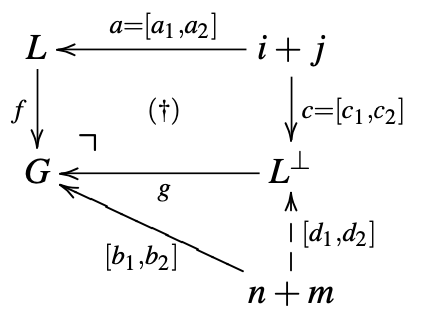
\includegraphics[width=0.3\linewidth]{figures/combinatorial_semantics/boundary_complement.png}
%     \label{fig:boundary_complement}
% \end{figure}

% is called a boundary complement if $[c_1, c_2]$ is mono and there exist $d_1 : n \to L^{\bot}$ and $d_2 : m \to L^{\bot}$ making the above triangle commute and such that
% \[
%     n + j \xrightarrow{[d_1,c_2]} L^{\bot} \xleftarrow{[d_2,c_1]} m + i
% \]
% is a monogamous cospan
% \end{definition}

\subsection{Syntactic rewriting of PROPs}

\Aleksei{Should this be a separate section rather than a subsection?}

\begin{definition}[\cite{Frobenius}]
A rewriting system $\mathcal{R}$ in a PROP $\mathbb{A}$ consists of a set of rewriting rules, i.e. pairs $\langle l , r \rangle$ of morphisms $l , r : i \to j$ in $\mathbb{A}$ with the same arities and co-arities. Given $a, b : m \to n$ in $\mathbb{A}$, $a$ rewrites into $b$ via $\mathcal{R}$, written $a\Rightarrow_{\mathcal{R}} b$ ,if they are decomposable as follows, for some rule $\langle l,r \rangle \in \mathcal{R}$    
\end{definition}

\begin{figure}[h!]
    
    \[
    \scalebox{0.75}{\tikzfig{combinatorial_semantics/prop_rewriting}}
    \]
\end{figure}

\begin{definition}
Given a rewriting system $\mathcal{R}$ for a $\textsf{PROP}(\Sigma)$ we define 
 a rewriting system $\mathcal{R}^{+}$ in a $\textsf{PROP}^{+}(\Sigma)$  as a set of pairs $\langle l , r \rangle$ for each pair $\langle l, r \rangle$ in $\mathcal{R}$.
However, the rewriting happens modulo semilattice enriched laws rather than SMC laws. We define what $a \Rightarrow_{\mathcal{R}^+} b$ means for some rule $\langle l , r\rangle $ based on the structure of $a$ and $b$.

If they are decomposable as above then we say that $a$ rewrites to $b$ under rule $\langle l, r \rangle$ in $\mathcal{R}^{+}$. Another case is when some $a'$ rewrites to some $b'$ under rule $\langle l, r \rangle$ in the sense above and then we say that $a$ rewrites to $b$ under the same rule if they are decomposable as below.

\begin{figure}

    \[
    \scalebox{0.6}{
    \tikzfig{combinatorial_semantics/prop_plus_rewriting}
    }
    \]
\end{figure}

\end{definition}



% \update{

% \begin{definition}
%     Functor $\llbracket \cdot \rrbracket : \text{PROP}^{+} \to \catname{MACsp_{D}(EHyp_{\Sigma})}$.

%     We will build this functor inductively. As noted above, $\MdaCospans$ is a full subcategory of $\catname{MACsp_{D}(EHyp_{\Sigma})}$ and the acting of this functor on generators can be found in~\cite{Frobenius}. We need to define what $+$ from $\text{PROP}^{+}$ in $\catname{MACsp_{D}(EHyp_{\Sigma})}$ is. The definition could be found in Figure~\ref{fig:f+g} where well-typed mda-cospans for images of arbitrary morphisms $f, g : m \to n$ are depicted on the left and the image of $f + g$ is depicted on the right. A new edge is introduced which is the immediate predecessor of arbitrary e-hypergraphs $f$ and all edges and nodes of $f$ and $g$ are in conflict. The nodes are added to the interfaces and to the new edge to preserve well-typedness.

% \end{definition}

% }





We will later mimic rewrites in $\textsf{PROP}^{+}(\Sigma)$ at the level of $\WellTypedMdaEcospans$ by utilising a generalisation of double-pushout with interfaces (DPOI) approach defined in~\cite{Frobenius}. First, we will recall standard double-pushout (DPO) rewriting.

DPO is a technique for formalising rewriting in graph-like categories. For a given rewrite rule $\langle l, r \rangle$ it corresponds to an intuitive notion of removing an occurrence of $l$ within a graph and then plugging $r$ in there. More specifically, a DPO rule is a span $L \xleftarrow{} K \xrightarrow{} R$ in some category $\mathcal{C}$ with pushouts, where $L$ stands for the $l$ part of a rewrite rule, $R$ stands for the $r$, and $K$ is the invariant that should be maintained during rewriting.

A typical DPO square looks like this


\[
\begin{tikzcd}
L \arrow[d, "m"'] & K \arrow[d] \arrow[l, "f"'] \arrow[r, "g"] & R \arrow[d]   \\
G^{\urcorner}     & C \arrow[l] \arrow[r]                      & ^{\ulcorner}H
\end{tikzcd}
\]

where the two marked squares are pushouts. Morphisms $K \to C \to G$ are called a \textit{pushout complement} and morphism $m$ is called a \textit{match} and is defined when the corresponding pushout complement exists. When $f,g$ are injective, constructing $C$ can be intuitively understood as finding an occurrence of $L$ in $G$ and removing from this occurrence everything that has no pre-image in $K$ and then inserting in there everything from $R$ that has no pre-image in $K$ (hence the two pushouts: one for deletion and one for insertion). Then we say that $G$ is rewritten into $H$ under a rewrite rule $L \xleftarrow{} K \xrightarrow{} R$. 

However, this notion of DPO does not account for hypergraphs with interfaces, i.e. those from $\MdaCospans$ where $l,r$ from $\langle l, r \rangle$ are cospans. To support this we first assume that we only need to maintain the interfaces of $i \xrightarrow{} L \xleftarrow{} j$ and $i \xrightarrow{} R \xleftarrow{} j$ during rewriting, then we can take $K \cong i + j$, i.e. take $K$ to be the coproduct of $i,j$ (remark 3.14~\cite{Frobenius}). What remains is to account for the interfaces in $G$, $C$, and $H$, which brings us to the following modified DPOI square. $J \cong n + m$ where $n$ and $m$ are the input and output interfaces of $G$, $C$, and $H$ respectively. The only difference from DPO square above is that we now explicitly require that the initial object $G$, intermediate object $C$ and final object $H$ all share the same interfaces.


\[
\begin{tikzcd}
L \arrow[d, "m"'] & K \arrow[d] \arrow[l, "f"'] \arrow[r, "g"] & R \arrow[d]   \\
G^{\urcorner}     & C \arrow[l] \arrow[r]                      & ^{\ulcorner}H \\
                  & J \arrow[lu] \arrow[u] \arrow[ru]          &              
\end{tikzcd}
\]

To mimic rewrites in $\textsf{PROP}(\Sigma)$ we need to put some restrictions on pushout complements as not all of them lead to mda-cospans.

\begin{definition}[Boundary complement for $\catname{MACsp_{D}(Hyp_{\Sigma}))}$]
\label{def:boundary_original}
For monogamous cospans $i \xrightarrow{a_1} L \xleftarrow{a_2} j$ and $n \xrightarrow{b_1} G \xleftarrow{b_2} m$
and mono $f : L \to G$, a pushout complement as depicted below

\begin{figure}[h!]
    \centering
    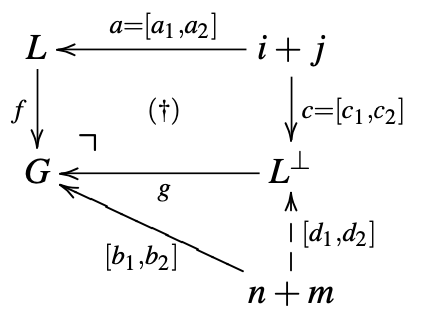
\includegraphics[width=0.3\linewidth]{figures/combinatorial_semantics/boundary_complement.png}
\end{figure}

is called a boundary complement if $[c_1, c_2]$ is mono and there exist $d_1 : n \to L^{\bot}$ and $d_2 : m \to L^{\bot}$ making the above triangle commute and such that
\[
    n + j \xrightarrow{[d_1,c_2]} L^{\bot} \xleftarrow{[d_2,c_1]} m + i
\]
is a monogamous cospan. 
\end{definition}

Intuitively, such a pushout complement requires that inputs get only glued to outputs and vice-verse in the two pushout squares.

\begin{definition}{Convex match}

We call a match $m : L \to G$ convex if it is mono and its image is a convex subgraph of $G$. 
    
\end{definition}

\begin{definition}{Rewriting in $\catname{MACsp_{D}({Hyp_{\Sigma}})}$}

Given $G \xleftarrow{} n+m$ and $H \xleftarrow{} n + m$ in $\catname{Hyp_{\Sigma}}$, $G$ rewrites convexly into $H$ with interface $n + m$ --- notation $(G \xleftarrow{} n + m ) \Rrightarrow_{\mathcal{R}}  (H \xleftarrow{} n + m )$ --- if there exist rule $L \xleftarrow{} i + j \xrightarrow{} R$ in $\mathcal{R}$ and object $C$ and cospan arrows $i+j \xrightarrow{} C \xleftarrow{} n+m$ in $\catname{Hyp_{\Sigma}}$ such that the DPOI diagram above commutes and its marked squares are pushouts and the following conditions hold

\begin{itemize}
    \item $m : L \to G$ is a convex match;
    \item $i + j \to C \to G$ is a boundary complement in the leftmost pushout.
\end{itemize}
    
\end{definition}

\begin{theorem}[Theorem 35~\cite{Frobenius2}]
    Let $R$ be any rewriting system on $\textsf{PROP}(\Sigma)$. Then,
    \[
    g \Rightarrow_{\mathcal{R}} h \;\text{ iff }\; \llbracket ^{\ulcorner}g^{\urcorner} \rrbracket \Rrightarrow_{\llbracket \mathcal{R} \rrbracket} \llbracket ^{\ulcorner}h^{\urcorner} \rrbracket 
    \]

    where $\llbracket \cdot \rrbracket : \textsf{PROP}(\Sigma) \to \MdaCospans$ is a faithful monoidal functor.
\end{theorem}

\begin{remark}
    Note that even though $n \xrightarrow{} G \xleftarrow{} m$ and $0 \xrightarrow{} G \xleftarrow{} n + m$ are essentially isomorphic \update{(they are not technically isomorphic because they have different legs)}, the functor $\llbracket \cdot \rrbracket$ deals with arbitrary string diagrams (that have multiple inputs and multiple outputs) in $\textsf{PROP}(\Sigma)$ and interprets them as cospans $n \xrightarrow{} G \xleftarrow{} m$. However, there is a syntactic operation $\ulcorner \cdot \urcorner$ on $\textsf{PROP}(\Sigma)$ to translate between string diagrams with multiple inputs and outputs and string diagrams with only outputs.

    \[
\tikzfig{combinatorial_semantics/bending_wires}
    \]

    Now the left-hand and right-hand sides are equivalent in the sense that $f \Rightarrow_{\langle l, r \rangle} g$ if and only if $\ulcorner f \urcorner \Rrightarrow_{\langle \ulcorner l \urcorner, \ulcorner r \urcorner \rangle} 
 \ulcorner g \urcorner$ and the latter string diagram can be interpreted as $0 \xrightarrow{} G \xleftarrow{} n + m$ for which we defined rewriting above.
\end{remark}

\Aleksei{TODO: discuss this}

\Aleksei{This holds for boxes with bent wires, which require a compact closed structure. The proof for the "only if" direction refers to the result for rewriting in PROP + Frob and for the converse direction it uses decomposition lemma and isomorphism-ness of a functor $\llbracket \cdot \rrbracket$ (Theorem 25~\cite{Frobenius2})}

\Aleksei{At some point I forgot to make a grey shaded area for cospans. Need to fix this.}

We have a more general notion of interface and hence we need to adjust DPOI rewriting a little bit. The first issue is that interfaces are not preserved during rewriting, consider an example above which corresponds to a rewrite rule of $\langle f, f+g \rangle$.

\begin{figure}[t]
    \centering
    \[
    \scalebox{0.75}{\tikzfig{combinatorial_semantics/f_to_f_plus_g_example}}
    \]
\end{figure}

The input interface on the left-hand side of the rule is $\{1, 2\}$, while the input interface on the right-hand side of the rule is $\{1,2,5,6,7,8\}$. Note that the outermost interfaces are preserved.

Another concern is when we delete the occurrence of the left-hand side of a rewrite rule from an e-hypergraph we also modify this e-hypergraph's interfaces. Consider a hypothetical DPO square below in Figure~\ref{fig:interface_change_example} where long arrows denote matching between carriers of cospans.

\begin{figure}
    \centering
    \[
    \scalebox{0.5}{\tikzfig{combinatorial_semantics/interfaces_change_example}}\]
    \caption{Hypothetical DPO square for $\catname{MACsp_{D}(EHyp_{\Sigma})}$}
    \label{fig:interface_change_example}
\end{figure}

The first row of the diagram shows the span for a rewrite rule of $\langle f + g, f \rangle$ which is like a projection rule. Note once again the difference between the interfaces of the left-hand and right-hand sides of the rewrite rule. The entry in the middle of the span depicts the outermost interfaces which are preserved. The second row depicts the e-hypergraph to be rewritten on the left and the result of the rewrite on the right. The result is obtained by first deleting the image of the left-hand side of the rewrite rule from the initial e-hypergraph (depicted in the middle) and then gluing the right-hand side of the rewrite rule into it. Note that the interfaces of the initial e-hypergraph and the residual e-hypergraph are different. Here, the outermost and the whole interfaces for the eventual e-hypergraph coincide, but if the nested-ness of the initial e-hypergraph was more intense the result could have inner interfaces as well as we would remove the interfaces of the inner edges when deleting the image of the left-hand side part of the rule from the initial e-hypergraph.

\Aleksei{TODO: show that there exists a pushout for each of the axioms and lifted rewrites}

\question{Shall I replace $i,j$ etc. with $X_{ext}$?}

To account for such changes in the interfaces we put some additional constraints on DPOI rewriting. Consider a DPOI diagram with extra constraints below.

% \[\begin{tikzcd}
% 	&&&& {i + j} \\
% 	{l_i+l_o} && L &&&& R && {r_i+r_o} \\
% 	\\
% 	{g_i+g_o} && {G^{\urcorner}} && C && {^{\ulcorner}H} && {h_i+h_o} \\
% 	\\
% 	&&&& {n+m}
% 	\arrow[color={rgb,255:red,214;green,92;blue,92}, from=1-5, to=2-3]
% 	\arrow[color={rgb,255:red,214;green,92;blue,92}, from=1-5, to=2-7]
% 	\arrow["m", color={rgb,255:red,214;green,92;blue,92}, from=2-3, to=4-3]
% 	\arrow["{[i_c,j_c]}", color={rgb,255:red,214;green,92;blue,92}, from=1-5, to=4-5]
% 	\arrow[color={rgb,255:red,214;green,92;blue,92}, from=2-7, to=4-7]
% 	\arrow["{[n_c,m_c]}"', color={rgb,255:red,214;green,92;blue,92}, from=6-5, to=4-5]
% 	\arrow[color={rgb,255:red,214;green,92;blue,92}, from=4-5, to=4-7]
% 	\arrow[color={rgb,255:red,214;green,92;blue,92}, from=4-5, to=4-3]
% 	\arrow[color={rgb,255:red,214;green,92;blue,92}, from=6-5, to=4-3]
% 	\arrow[color={rgb,255:red,214;green,92;blue,92}, from=6-5, to=4-7]
% 	\arrow[from=2-1, to=2-3]
% 	\arrow["{[f_i,f_o]}", from=2-1, to=4-1]
% 	\arrow[from=4-1, to=4-3]
% 	\arrow[from=2-9, to=2-7]
% 	\arrow[from=4-9, to=4-7]
% 	\arrow["{[h_i,h_o]}"{description}, from=2-9, to=4-9]
% 	\arrow[from=6-5, to=4-9]
% 	\arrow[from=6-5, to=4-1]
% 	\arrow["{[i_l,j_l]}"{description}, from=1-5, to=2-1]
% 	\arrow["{[i_r,j_r]}"{description}, from=1-5, to=2-9]
% \end{tikzcd}\]


% https://q.uiver.app/#q=WzAsMTEsWzIsMSwiTCJdLFs0LDAsImkgKyBqIl0sWzIsMywiR157XFx1cmNvcm5lcn0iXSxbNCwzLCJDIl0sWzQsNSwibittIl0sWzAsMSwibF9pK2xfbyJdLFswLDMsImdfaStnX28iXSxbNiwxLCJSIl0sWzYsMywiXntcXHVsY29ybmVyfUgiXSxbOCwzLCJoX2kraF9vIl0sWzgsMSwicl9pK3JfbyJdLFsxLDAsIiIsMCx7ImNvbG91ciI6WzAsNjAsNjBdfV0sWzAsMiwibSIsMCx7ImNvbG91ciI6WzAsNjAsNjBdfSxbMCw2MCw2MCwxXV0sWzEsMywiW2lfYyxqX2NdIiwwLHsiY29sb3VyIjpbMCw2MCw2MF19LFswLDYwLDYwLDFdXSxbNCwzLCJbbl9jLG1fY10iLDIseyJjb2xvdXIiOlswLDYwLDYwXX0sWzAsNjAsNjAsMV1dLFszLDIsIiIsMix7ImNvbG91ciI6WzAsNjAsNjBdfV0sWzQsMiwiIiwyLHsiY29sb3VyIjpbMCw2MCw2MF19XSxbNSwwXSxbNiwyXSxbNCw2XSxbMSw1LCJbaV9sLGpfbF0iLDFdLFs0LDgsIiIsMCx7ImNvbG91ciI6WzAsNjAsNjBdfV0sWzMsOCwiIiwwLHsiY29sb3VyIjpbMCw2MCw2MF19XSxbNyw4LCIiLDIseyJjb2xvdXIiOlswLDYwLDYwXX1dLFsxLDcsIiIsMix7ImNvbG91ciI6WzAsNjAsNjBdfV0sWzEwLDddLFs5LDhdLFsxLDEwXSxbNCw5XV0=
\[\begin{tikzcd}
	&&&& {i + j} \\
	{l_i+l_o} && L &&&& R && {r_i+r_o} \\
	\\
	{g_i+g_o} && {G^{\urcorner}} && C && {^{\ulcorner}H} && {h_i+h_o} \\
	\\
	&&&& {n+m}
	\arrow[draw={rgb,255:red,214;green,92;blue,92}, from=1-5, to=2-3]
	\arrow["m", color={rgb,255:red,214;green,92;blue,92}, from=2-3, to=4-3]
	\arrow["{[i_c,j_c]}", color={rgb,255:red,214;green,92;blue,92}, from=1-5, to=4-5]
	\arrow["{[n_c,m_c]}"', color={rgb,255:red,214;green,92;blue,92}, from=6-5, to=4-5]
	\arrow[draw={rgb,255:red,214;green,92;blue,92}, from=4-5, to=4-3]
	\arrow[draw={rgb,255:red,214;green,92;blue,92}, from=6-5, to=4-3]
	\arrow[from=2-1, to=2-3]
	\arrow[from=4-1, to=4-3]
	\arrow[from=6-5, to=4-1]
	\arrow["{[i_l,j_l]}"{description}, from=1-5, to=2-1]
	\arrow[draw={rgb,255:red,214;green,92;blue,92}, from=6-5, to=4-7]
	\arrow[draw={rgb,255:red,214;green,92;blue,92}, from=4-5, to=4-7]
	\arrow[draw={rgb,255:red,214;green,92;blue,92}, from=2-7, to=4-7]
	\arrow[draw={rgb,255:red,214;green,92;blue,92}, from=1-5, to=2-7]
	\arrow[from=2-9, to=2-7]
	\arrow[from=4-9, to=4-7]
	\arrow[from=1-5, to=2-9]
	\arrow[from=6-5, to=4-9]
\end{tikzcd}\]

The original DPOI square is shown in red. The extra bits simply account for more complicated interfaces.
For example, the left-hand side $L$ of a rewrite rule $\langle L, R \rangle$ which originally was some cospan $i \xrightarrow{} L \xleftarrow{} j$ in $\MdaCospans$ now is a cospan $i \xrightarrow{} l_i \to L \xleftarrow{} l_o \xleftarrow{} j$ from $\WellTypedMdaEcospans$ where $l_i, l_o$ are whole input and output interfaces respectively.
The top half of this diagram says that the outermost interfaces should coincide for $L$ and $R$. The bottom half puts the same restrictions on $G$ and $H$. 
% The extra squares on both sides say that there should exist a matching of the interfaces together with a matching of e-hypergraphs. This requirement was implicit in the case of $\catname{MACsp_{D}(Hyp_{\Sigma}}$ because the whole interfaces and the outermost interfaces coincided. Because now the interfaces can change, we need to keep track of which parts of the interfaces are subjected to changes.


We also adjust the definition of a boundary complement a bit.

\begin{definition}[Boundary complement in $\WellTypedMdaEcospans$]
\label{def:boundary_new}

% https://q.uiver.app/#q=WzAsNyxbMiwxLCJMIl0sWzQsMCwiaSArIGoiXSxbMiwzLCJHXntcXHVyY29ybmVyfSJdLFs0LDMsIkMiXSxbNCw1LCJuK20iXSxbMCwxLCJsX2krbF9vIl0sWzAsMywiZ19pK2dfbyJdLFsxLDAsIiIsMCx7ImNvbG91ciI6WzAsNjAsNjBdfV0sWzAsMiwibSIsMCx7ImNvbG91ciI6WzAsNjAsNjBdfSxbMCw2MCw2MCwxXV0sWzEsMywiW2lfYyxqX2NdIiwwLHsiY29sb3VyIjpbMCw2MCw2MF19LFswLDYwLDYwLDFdXSxbNCwzLCJbbl9jLG1fY10iLDIseyJjb2xvdXIiOlswLDYwLDYwXX0sWzAsNjAsNjAsMV1dLFszLDIsIiIsMix7ImNvbG91ciI6WzAsNjAsNjBdfV0sWzQsMiwiIiwyLHsiY29sb3VyIjpbMCw2MCw2MF19XSxbNSwwXSxbNiwyXSxbNCw2XSxbMSw1LCJbaV9sLGpfbF0iLDFdXQ==
\[\begin{tikzcd}
	&&&& {i + j} \\
	{l_i+l_o} && L \\
	\\
	{g_i+g_o} && {G^{\urcorner}} && C \\
	\\
	&&&& {n+m}
	\arrow[color={rgb,255:red,214;green,92;blue,92}, from=1-5, to=2-3]
	\arrow["m", color={rgb,255:red,214;green,92;blue,92}, from=2-3, to=4-3]
	\arrow["{[i_c,j_c]}", color={rgb,255:red,214;green,92;blue,92}, from=1-5, to=4-5]
	\arrow["{[n_c,m_c]}"', color={rgb,255:red,214;green,92;blue,92}, from=6-5, to=4-5]
	\arrow[color={rgb,255:red,214;green,92;blue,92}, from=4-5, to=4-3]
	\arrow[color={rgb,255:red,214;green,92;blue,92}, from=6-5, to=4-3]
	\arrow[from=2-1, to=2-3]
	\arrow[from=4-1, to=4-3]
	\arrow[from=6-5, to=4-1]
	\arrow["{[i_l,j_l]}"{description}, from=1-5, to=2-1]
\end{tikzcd}\]
Consider the diagram above where the marked square is a pushout and $i + j$ and $n + m$ are the \textit{outermost} interfaces for cospans $i \xrightarrow{} l_i \xrightarrow{} L \xleftarrow{} l_o \xleftarrow{} j$ and $n \xrightarrow{} g_i \xrightarrow{} G \xleftarrow{} g_o \xleftarrow{} m$. We say that $i+j \to C \to G^{\urcorner}$ is a \textit{boundary} complement if $[i_c, i_j]$ is mono and there exist $n_c : n \to C$ and $m_c : m \to C$ making the above triangle commute and such that there exists a \textit{not necessarily well-typed} mda-cospan

\[
n \xrightarrow{} c_i + j \xrightarrow{} C \xleftarrow{} c_o + i \xleftarrow{} m
\]

where $c_i$ and $c_o$ are computed as $c_i = g_i \setminus (l_i \setminus i)$ and $c_o = g_o \setminus (l_o \setminus j)$.

% \Aleksei{The pushout interpretation is wrong because there might not be a morphism between $i$ and $c_i$ and similarly for $j$ and $c_o$. Any other categorical interpretation? The outermost interface of the rewrite span may not be a part of the interface of $G$}



% where $l_i + l_o$ is the whole interface for $L$, $g_i + g_o$ is the whole interface for $G$.
\end{definition}

% Intuitively, these pushout squares mean that when we delete the occurrence of $L$ from $G$ we also remove the occurrence of $L$'s interface within $G$'s interface preserving the outermost interfaces $i + j$. The highlighted arrows form the pushout square for the original boundary complement.

% We call morphisms $i + j \to C \to G$ a boundary complement if

% \begin{enumerate}
%     \item The square above commutes and $L \xrightarrow{} G \xleftarrow{} C$ is a pushout
%     \item There exists an mda cospan $g_i \setminus (l_i \setminus i) + j \xrightarrow{} C \xleftarrow{} g_o \setminus (l_o \setminus j) + i$. \question{I am unsure about categorical notation for this set difference. Maybe it can be paraphrased in the following way?}
%     \item There exists an mda cospan $c_i + j \xrightarrow{} C \xleftarrow{} c_o + i$ where $c_i$ and $c_o$ are the following pushout complements in the category of discrete hypergraphs:
% \end{enumerate}



% The second point above means that when cutting the mono-occurrence of $L$ out from $G$ we also need to remove the inner interfaces of $L$ from the whole interface of $G$. \question{According to the pushout squares above, $c_i$ is constructed by removing from $g_i$ everything from $l_i$ which does not have a pre-image in $i$, i.e., everything except the outermost interfaces (same holds for $c_o$)}

\begin{remark}
Note that cospan $n \xrightarrow{} c_i + j \xrightarrow{} C \xleftarrow{} c_o + i \xleftarrow{} m$ is not well-typed. The cospan's input interface contains nodes that previously were a part of the output interface.
\end{remark}

First, let's check that this notion generalises the ordinary boundary complement from~\ref{def:boundary_original}. For this, we assume that child and conflict relations are empty in which case $i + j$ and $l_i + l_o$ coincide as well as $g_i + g_o$ and $n + m$. Hence, $g_i \setminus (l_i \setminus i) + j = g_i + j = n + j$ and the same for the output interfaces. Thus we have $n + j \xrightarrow{} C \xleftarrow{} m + i$, which corresponds to the definition from~\ref{def:boundary_original}.

% Next, consider an example from figure~\ref{fig:dpoir}. The outermost interfaces of $L$ coincide with the whole interfaces, i.e. $l_i + l_o = i + j$. However, $n + m = \{0'', 1''\}$ and $g_i + g_o = \{0'',0,2,1,3,1''\}$. According to the definition of a boundary complement the following mda cospan should exist: $g_i \setminus (l_i \setminus i) + j = \{0'', 0, 2\} \setminus \varnothing \cup \{1\} = \{0'',0,2,1\} \xrightarrow{} C \xleftarrow{} \{0,1,3,1''\} = \text{same procedure for output interfaces}$.

% \question{We need to show that this boundary complement is unique and that after performing a pushout on the right the result is also an mda hypergraph}

% We can now present a complete DPOI square

% \[
% \begin{tikzcd}
%                    &                    & i+j \arrow[ld] \arrow[lld] \arrow[ddd, "f"] \arrow[rrd] \arrow[rd] &                    &              &  &                       &               &                       &               \\
% L \arrow[dd, "m"'] & l_i+l_o \arrow[l]  &                                                                    & r_i+r_j \arrow[r]  & R \arrow[dd] &  & i \arrow[r] \arrow[d] & r_i \arrow[d] & j \arrow[d] \arrow[r] & r_o \arrow[d] \\
%                    &                    &                                                                    &                    &              &  & c_i \arrow[r]         & h_i           & c_o \arrow[r]         & h_o           \\
% G                  &                    & C \arrow[ll] \arrow[rr]                                            &                    & H            &  &                       &               &                       &               \\
%                    & g_i+g_o \arrow[lu] & n+m \arrow[u] \arrow[l] \arrow[llu] \arrow[r] \arrow[rru]          & h_i+h_o \arrow[ru] &              &  &                       &               &                       &              
% \end{tikzcd}
% \]



% \begin{remark}
%     Note that in all pushout squares for the interfaces all the morphisms are monos. \question{Does it follow from anything above? Because the corresponding triangles commute?}
% \end{remark}



\begin{proposition}
    The boundary complement in~\ref{def:boundary_new} when exists is unique
    \begin{proof}
        \update{TODO}
    \end{proof}
\end{proposition}


\question{
\begin{definition}[Convex down-closed conflict reflecting match] 
    We call $m : L \to G$ in $\catname{EHyp_{\Sigma}}$ a convex down-closed conflict reflecting match if
    
    \begin{enumerate}
        \item $m$ is monomorphism
        \item $m(L)$ is a convex down-closed subgraph of $G$
        \item if $m(x_1) \# m(x_2)$ then $x_1 \# x_2$
    \end{enumerate}
\end{definition}
}


\begin{definition}[Rewriting in $\WellTypedMdaEcospans$]
    Given $G \xleftarrow{} g_i + g_o \xleftarrow{} n + m$ and $H \xleftarrow{} h_i + h_o \xleftarrow{} n+m$ in $\WellTypedMdaEcospans$ with the outermost interfaces $n + m$, $G$ rewrites convexly into $H$ with the outermost interface $n + m$ --- notation $( G \xleftarrow{} n + m ) \Rrightarrow_{\mathcal{R}} (E \xleftarrow{} n + m )$ --- if there exists a rule $l_i + l_o \xrightarrow{} L \xleftarrow{} i + j \xrightarrow{} R \xleftarrow{} r_i + r_o$ with the outermost interfaces $i+j$ in $\mathcal{R}$ and object $C$ and cospan arrows $i+j \xrightarrow{} C \xleftarrow{} n+m$ in $\Ecospans$ such that the diagram below commutes and its marked squares are pushouts

% https://q.uiver.app/#q=WzAsMTEsWzIsMSwiTCJdLFs0LDAsImkgKyBqIl0sWzIsMywiR157XFx1cmNvcm5lcn0iXSxbNCwzLCJDIl0sWzQsNSwibittIl0sWzAsMSwibF9pK2xfbyJdLFswLDMsImdfaStnX28iXSxbNiwxLCJSIl0sWzYsMywiXntcXHVsY29ybmVyfUgiXSxbOCwzLCJoX2kraF9vIl0sWzgsMSwicl9pK3JfbyJdLFsxLDAsIiIsMCx7ImNvbG91ciI6WzAsNjAsNjBdfV0sWzAsMiwibSIsMCx7ImNvbG91ciI6WzAsNjAsNjBdfSxbMCw2MCw2MCwxXV0sWzEsMywiW2lfYyxqX2NdIiwwLHsiY29sb3VyIjpbMCw2MCw2MF19LFswLDYwLDYwLDFdXSxbNCwzLCJbbl9jLG1fY10iLDIseyJjb2xvdXIiOlswLDYwLDYwXX0sWzAsNjAsNjAsMV1dLFszLDIsIiIsMix7ImNvbG91ciI6WzAsNjAsNjBdfV0sWzQsMiwiIiwyLHsiY29sb3VyIjpbMCw2MCw2MF19XSxbNSwwXSxbNiwyXSxbNCw2XSxbMSw1LCJbaV9sLGpfbF0iLDFdLFs0LDgsIiIsMCx7ImNvbG91ciI6WzAsNjAsNjBdfV0sWzMsOCwiIiwwLHsiY29sb3VyIjpbMCw2MCw2MF19XSxbNyw4LCIiLDIseyJjb2xvdXIiOlswLDYwLDYwXX1dLFsxLDcsIiIsMix7ImNvbG91ciI6WzAsNjAsNjBdfV0sWzEwLDddLFs5LDhdLFsxLDEwXSxbNCw5XV0=
\[\begin{tikzcd}
	&&&& {i + j} \\
	{l_i+l_o} && L &&&& R && {r_i+r_o} \\
	\\
	{g_i+g_o} && {G^{\urcorner}} && C && {^{\ulcorner}H} && {h_i+h_o} \\
	\\
	&&&& {n+m}
	\arrow[draw={rgb,255:red,214;green,92;blue,92}, from=1-5, to=2-3]
	\arrow["m", color={rgb,255:red,214;green,92;blue,92}, from=2-3, to=4-3]
	\arrow["{[i_c,j_c]}", color={rgb,255:red,214;green,92;blue,92}, from=1-5, to=4-5]
	\arrow["{[n_c,m_c]}"', color={rgb,255:red,214;green,92;blue,92}, from=6-5, to=4-5]
	\arrow[draw={rgb,255:red,214;green,92;blue,92}, from=4-5, to=4-3]
	\arrow[draw={rgb,255:red,214;green,92;blue,92}, from=6-5, to=4-3]
	\arrow[from=2-1, to=2-3]
	\arrow[from=4-1, to=4-3]
	\arrow[from=6-5, to=4-1]
	\arrow["{[i_l,j_l]}"{description}, from=1-5, to=2-1]
	\arrow[draw={rgb,255:red,214;green,92;blue,92}, from=6-5, to=4-7]
	\arrow[draw={rgb,255:red,214;green,92;blue,92}, from=4-5, to=4-7]
	\arrow[draw={rgb,255:red,214;green,92;blue,92}, from=2-7, to=4-7]
	\arrow[draw={rgb,255:red,214;green,92;blue,92}, from=1-5, to=2-7]
	\arrow[from=2-9, to=2-7]
	\arrow[from=4-9, to=4-7]
	\arrow[from=1-5, to=2-9]
	\arrow[from=6-5, to=4-9]
\end{tikzcd}\]
    and the following conditions hold

    \begin{enumerate}
        \item $m : L \to G$ is a convex down-closed conflict reflecting match;
        \item $i + j \to C \to G$ is a boundary complement in the leftmost pushout.
    \end{enumerate}
\end{definition}

% \Aleksei{We may need the following proofs:}
% \begin{itemize}
%     \item The existence of pushout complements (for rewriting)
%     \item Soundness and completeness, that is the correspondence between enriched terms and e-hypergraphs.
%     \item Rewriting
%     \item Anything else?
% \end{itemize}

\Aleksei{Do we need to introduce substitution? This is needed if our rewrite rules are going to have variables as labels.}


The whole interfaces of the resulting e-hypergraph $H$ from the cospan $n \xrightarrow{} h_i \xrightarrow{} H \xleftarrow{} h_o \xleftarrow{} m$ are constructed as $h_i = (r_i \setminus i) + c_i$ and $h_o = (r_o \setminus j) + c_o$. $h_i \to H$ is defined as a copairing of $f_1 : r_i \setminus i \to R \to H$ and $f_2 : c_i \to C \to H$. Since both $f_1$ and $f_2$ are mono, their copairing is also a mono. Similarly for $h_o$.

% using the two pushout squares below.
% Intuitively, these squares combine the interfaces of $R$ and $C$ and identify those bits that share the same pre-image in the outermost interface $i + j$.

% \[\begin{tikzcd}
% i \arrow[r] \arrow[d] & r_i \arrow[d] & j \arrow[r] \arrow[d] & r_o \arrow[d] \\
% c_i \arrow[r]         & h_i           & c_o \arrow[r]         & h_o          
% \end{tikzcd}\]

% Going back to the example from the figure~\ref{fig:dpoir}, $h_i = \{0'',0,0',2',2\}$, $r_i = \{0,0',2'\}$, $r_o = \{1',3',1\}$, $h_o = \{1',3',3,1,1''\}$, $c_i = \{0'',2,0\}$, $c_o = \{1'',1,3\}$, $i = \{0\}$, $j = \{1\}$, where $h_i$ is exactly $c_i \coprod_{\equiv_{i}} r_i = \{0'',2,0\} \coprod_{\equiv_{i}} \{0,0',2'\} = \{0'',0,0',2',2\}$ and the same for $h_o$. 

\begin{proposition}

$n \xrightarrow{n_h} h_i \xrightarrow{f} H \xleftarrow{g} h_o \xleftarrow{m_h} m$ is a well-typed mda-cospan.

\begin{proof}
$f$ and $g$ are monos by construction. $n + m \to h_i + h_o$ is a mono by commutativity because $n + m \to H$ is a mono (also by commutativity). 
The only in-degree 0 nodes have a pre-image in $c_i$ and $r_i \setminus i$  and end up being in the image of $h_i$ (the nodes with the pre-image in $j$ get are glued together). Well-typedness is restored once the right-hand side of the rewrite rule is glued into $C$.  \question{Uniqueness of this pushout complement? Is it a presheaf? As a presheaf category is adhesive, $\catname{Csp_{D}(EHyp)}$ can not be a presheaf as it is not adhesive.}
\end{proof}
\end{proposition}

\Aleksei{Check the proof
}

\begin{lemma}(Decomposition). Let $m \xrightarrow{} G \xleftarrow{} n$ be a monogamous acyclic cospan and $L$ a convex and down-closed sub-hypergraph of $G$. Then there exists $k \in \mathcal{N}$ and a unique cospan $i \xrightarrow{} L \xleftarrow{} j$ such that G factors as $\ldots$

\update{TODO: this lemma is needed to prove soundness of rewriting}
\end{lemma}

\Aleksei{Can we reuse anything from~\cite{Frobenius}?}


Consider an example below that illustrates the introduced constraints.

\begin{remark}
    For now, we will informally denote a combinatorial interpretation of a morphism $f$ in $\textsf{PROP}^{+}(\Sigma)$ as $\llbracket f \rrbracket$.
\end{remark}

\begin{example}

A DPOI square for rewriting in $\WellTypedMdaEcospans$ is depicted in Figure~\ref{fig:refined_dpoi}.
A projection rule of $\llbracket f + g \rrbracket \to \llbracket f \rrbracket$ is shown in the top half of the diagram.
The image of the matching $m$ is shown in red and its image is a convex down-closed e-hypergraph.
Pushout complement is then computed by removing the image of $m$ from the target e-hypergraph by keeping intact the nodes that have a pre-image in the carrier of the rewriting span. The corresponding mda-cospan is depicted at the bottom: $c_i = g_i \setminus (l_i \setminus i) = \{18, 19, 1, 2, 13, 14, 5, 6, 7, 8\} \setminus (\{1,2,5,6,7,8\} \setminus \{1,2\}) = \{18, 19, 1, 2, 13, 14, 5, 6, 7, 8\} \setminus \{5,6,7,8\} = \{18,19,1,2,13,14\}$ and $c_i + j = \{18,19, 1, 2, 13, 14, 3, 4\}$ which is the input interface for $C$. Similar computations are performed for $c_o$. Then pushout glues $R$ and $C$ together along $i + j$ and the resulting interface $h_i = c_i + (r_i \setminus i) = \{18,19, 1, 2, 13, 14\} + \varnothing = \{18,19, 1, 2, 13, 14\}$ and likewise for $h_o$.

%     \begin{figure}
%         \centering
% \[
%   \scalebox{0.3}{      \tikzfig{combinatorial_semantics/refined_dpoi_example}
% }
%         \]
%     \caption{Refined DPOI rewriting}
%     \label{fig:refined_dpoi}
%     \end{figure}
    
\end{example}

\Aleksei{This figure yeilds "Dimension too large". Need to fix it.}

Unlike SMC equations the equations for semilattice enriched categories are not absorbed by e-hypergraph representation and hence to further build a correspondence between $\textsf{PROP}^{+}(\Sigma)$ and $\WellTypedMdaEcospans$ we add them as structural rewrite rules into $\llbracket \mathcal{R}^+ \rrbracket$. Recall that the category $\catname{EHyp_{\Sigma}}$ does not have all pushouts and hence we need to explicitly show that the pushouts that we need exist.


\begin{proposition}
Pushouts for all semilattice enrichment equations exist.

\begin{proof}
    Let us give a combinatorial interpretation for an instance of the first equation (distributivity) in~\ref{fig:string-equations}. It can be found in Figure~\ref{fig:distributivity_interpretation}. After we identify a convex down-closed image of the left-hand side of this rule within a graph $G$ we remove the image by keeping only the outermost nodes. Then we simply glue the right-hand side of the rule into the hole. Since we glue along the outermost nodes this does not introduce any conflict with regard to child relation. Such equations are not absorbed by e-hypergraph representation unlike SMC equations because the right-hand side contains more edges.

\end{proof}
\end{proposition}

\update{I think I haven't paid any attention to this fact previously, but it seems that in~\cite{Frobenius} the functor $\llbracket - \rrbracket$ is between $PROP_{\Sigma_{Frob}}$ and $Csp_{D}(Hyp_{\Sigma})$, i.e. PROP is quotiented by Frobenius equations, but they are absorbed in hypergraphs domain. We will have a similar thing: $\llbracket - \rrbracket: PROP^{+}_{\Sigma^{+}} \to \WellTypedMdaEcospans_{R^+}$, i.e. we will quotient PROP$^{+}$ by semilattice equations and quotient e-hypergraphs by the interpretation of these equations as they are not absorbed. The quotienting on the left is always implicit?}

\begin{figure}
    \centering
    \[
    \scalebox{0.45}{
    \tikzfig{combinatorial_semantics/structural_rule_pushout}}\]  
    \caption{Distributivity rewrite rule interpretation}
    \label{fig:distributivity_interpretation}
\end{figure}

\begin{definition}
    We will denote $\llbracket \mathcal{E} \rrbracket$ the interpretation of the equations in~\ref{fig:string-equations} as rewrite rules in $\WellTypedMdaEcospans$. In particular, for all $l = r$ in $\mathcal{E}$ $\llbracket \mathcal{E} \rrbracket$ will contain $\langle \llbracket l \rrbracket, \llbracket r \rrbracket \rangle$ and $\langle \llbracket r \rrbracket, \llbracket l \rrbracket \rangle$. \update{Technically we add those for all input and output interfaces.}
\end{definition}


\begin{remark}
    There is a minor limitation for DPOI rewriting above. It is unable to express rewriting for rules that contain an edge with no inputs and outputs on their right-hand side. This is because there is no way to impose both conflict and child relation of such an edge as it has no incident nodes in its context. An example of this could be seen in Figure~\ref{fig:non_expressible}. After an image of a match is removed there is no way of plugging $k$ into the hierarchical edge as it has no connection with this edge via the shared interface. However, we think that this is only a minor limitation because in practice such edges with no incident nodes correspond to `scalars' if we consider for example a category of vector spaces where a rewrite rule with a scalar could be

\begin{alignat*}{3}
\begin{pmatrix}
 1 &  2 \\
-1 &  1 \\
\end{pmatrix}
&\!\begin{aligned}
\hspace{1em} & \otimes &
\end{aligned}
&\!\begin{aligned}
2 &
\end{aligned}
&\!\begin{aligned}
 & \xrightarrow{} & 
\end{aligned}
&\!\begin{aligned}
\begin{pmatrix}
 2 &  4 \\
-2 &  2 \\
\end{pmatrix}    
\end{aligned}
\end{alignat*}
\end{remark}

That is, typically such scalars are absorbed and not present on the right-hand side of a rewrite rule.

\begin{figure}
    \centering
\[
\scalebox{0.5}{
\tikzfig{combinatorial_semantics/non_expressible_rewrite}
}
\]
    \caption{Non expressible rewrite}
    \label{fig:non_expressible}
\end{figure}

\newpage